\chapter{The Experimental Apparatus}\label{ch:ExptApp}

The Large Hadron Collider (LHC)~\cite{Brüning:782076,Evans:2008zzb} is the world's highest energy particle accelerator and collider, situated
at the European Organization for Nuclear Research (CERN), on the French-Swiss border near Geneva, Switzerland. The Compact Muon Solenoid 
(CMS)~\cite{Chatrchyan:2008aa} experiment is one of the two general purpose detectors that measures the properties of particles produced 
from proton-proton (\pp) and heavy-ion collisions at the LHC. This chapter briefly describes the details of the design and performance 
of the CERN accelerator complex and the CMS experiment.

\section{The Large Hadron Collider}
In the last few decades, the standard model of particle physics has been tested experimentally to excellent precision and is a well established theory
explaining the interactions of the fundamental particles. Many of these precise measurements were carried out at the Large Electron-Positron
 (\gls{LEP}) collider at CERN. As suggested by the de Broglie relation, $\Delta\text{}E\cdot\Delta{x}\simeq{\hbar}$, to probe increasingly smaller 
constituents, higher and higher energy is required. The maximum energy that can be attained by a particle orbiting in a circular path is limited by the 
energy loss due to synchrotron radiations given by
\begin{equation}
-\Delta{E} = \frac{4\pi\alpha}{3r}\beta^{3}\gamma^{4}
\label{eq:synRadn}
\end{equation}
where $r$ is the radius of circular path, $\beta=v/c\approx1$, as particles travel with velocity very close to the speed of light and $\gamma=E/mc^{2}$
with $m$ being mass of the accelerated particles. This synchrotron effect can be reduced either by increasing the radius of the collider (a linear
one would be optimal) or by using heavier particles. For financial reasons, there was a strong motivation to re-use the the LEP tunnel. Thus, 
according to \eqn{\ref{eq:synRadn}}, the other efficient way to increase center-of-mass energy is to increase the mass of the accelerated particles, 
\ie, protons for LHC. Since the rest mass of protons is about 2000 times more than the rest mass of electrons, the energy loss due to synchrotron 
radiation for protons is decreased by a factor of (2000)$^{4}\approx10^{13}$ compared to that of electrons.
%The LHC could have also considered colliding proton anti-proton instead of proton proton but with the later choice, it is almost impossible to attain the intensity LHC need to search for rare processes.
The LHC is also designed to include the heavy ion collisions but the differences in proton and ion beams on various aspects limit the luminosity and 
beam lifetime~\cite{Evans:2008zzb}.

As protons are not elementary particles but have a sub-structure, \pp collision phenomenology is very different from lepton collisions. A proton 
is made up of constituent partons $-$ quarks and gluons, with a given constituent carrying only a fraction of the total proton energy. In a collision, 
typically only one each of the parton are engaged in a hard scattering process with the effective center-of-mass energy of the hard scattering, 
$\sqrt{\hat{s}}$, being determined by the momentum fractions $x_{1}$, $x_{2}$ carried by partons, and given by $\sqrt{\hat{s}}=\sqrt{x_{1}x_{2}s}$, 
where $\sqrt{s}$ is the center-of-mass energy of proton beams. In each proton-proton collision there is a probability to produce different process 
depending on its cross section and momentum exchange between the colliding partons.

The LHC~\cite{Evans:2008zzb,Brüning:782076} is a two ring superconducting accelerator and collider, located in the 27\unit{km} circular underground 
tunnel originally built for the LEP collider on the French-Swiss border. The tunnel has a diameter of 3.7\unit{m} and the depth varies between 
50\unit{m} and 175\unit{m} (according to the land topology). It houses a twin-bore magnet which provides a magnetic field to both the proton beams in 
the same structure. To keep the proton beams on track, a magnetic field of 8.3\unit{T} is needed, which is achieved by using superconducting dipole 
magnets operating at a temperature of $1.9^{^{\circ}}$\unit{K}. About 37 million Kg of superfluid Helium is used to cool the Niobium-Titanium windings 
of the magnets to reach the superconducting state. The LHC has 1232 dipole magnets each of which weights 30\unit{tonnes} and is 15\unit{m} long. The 
LHC is also installed with eight Radio Frequency (RF) cavities for each beam to correct for the synchrotron radiation losses. These cavities operate at 
$4.5^{^{\circ}}$\unit{K}, with each cavity delivering  2\unit{MV} at 400\unit{MHz}.

\begin{figure}[h!]
\centering
\includegraphics[width=18cm,height=10cm]{ch2/figures/CERN-Accelerator-Complex.jpg}
\caption{Picture showing the LHC ring and a series of accelerators which boost the proton (ion) beam to different energy levels~\cite{Web:CERN}.}
\label{fig:CERNAccComplex}
\end{figure}
Before two proton beams collide in the LHC at the desired center-of-mass energy, the beams have to be accelerated in several steps, as with the
presently available resources, it is experimentally challenging to reach an energy of 4\unit{TeV} (or designed 7\unit{TeV}) per beam in a single step.
Protons are first accumulated using hydrogen atoms contained in a simple bottle of hydrogen gas after stripping off electrons by applying an
electric field. Protons are then accelerated in \gls{LINAC2}, a linear accelerator consisting of RF cavities, to an energy of 50\unit{MeV}. These are 
then transferred to the Proton Synchrotron Booster (\gls{PSB}), which accelerates the beam to 1.4\unit{GeV}. Then the proton beams
are accelerated up to 25\unit{GeV} in the Proton Synchrotron (\gls{PS}) and up to 450\unit{GeV} in the Super Proton Synchrotron (\gls{SPS}). 
Finally, these are injected into the LHC rings and accelerated to an energy of 4\unit{TeV} resulting in a center-of-mass energy 
of 8\unit{TeV}. The entire CERN accelerator complex houses several experiments and facilities as illustrated in \fig{\ref{fig:CERNAccComplex}}.
Details of these can be found in Ref.~\cite{Web:CERN}. 

\begin{figure}[h!]
\centering
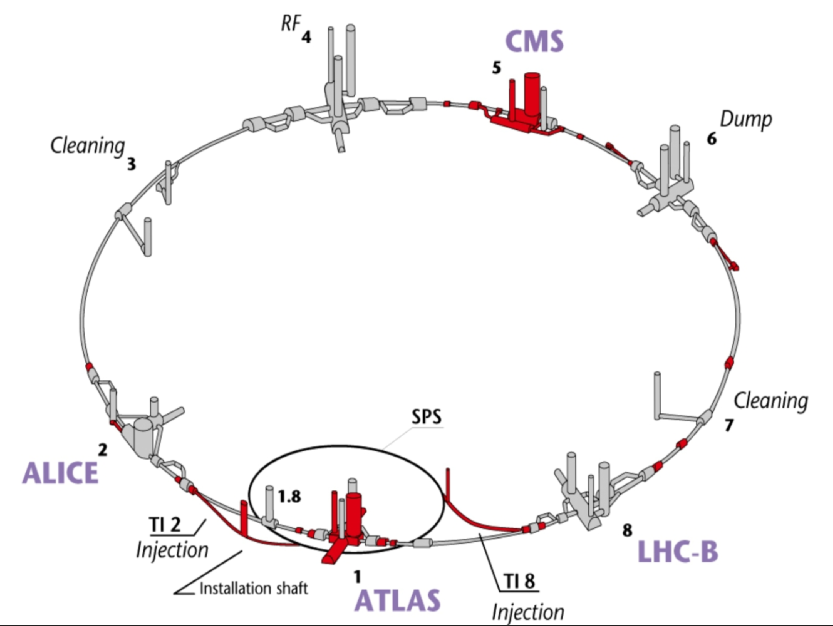
\includegraphics[width=10cm,height=8cm]{ch2/figures/lhcLayout_v2.png}
\caption{Layout of LHC ring~\cite{Web:CERNcds}.}
\label{fig:lhcLayout}
\end{figure}

The LHC tunnel is geometrically organized in eight crossing points, flanked by eight straight sections, and arcs. Each straight section has a 
length of 528\unit{m} and can serve as an experimental insertion, a point where two beams travelling in opposite directions can collide. A schematic 
representation of the LHC tunnel is depicted in \fig{\ref{fig:lhcLayout}}. The insertion points are labeled with 
integer numbers increasing in counter-clockwise direction. The LHC hosts four major detectors. A Toroidal LHC ApparatuS (ATLAS)~\cite{atlasTDR} and 
Compact Muon Solenoid (CMS)~\cite{cmsTDR} are the two general purpose detectors situated at points 1 and 5 insertion regions respectively. At point 2 
and 8 lie respectively, the experiments, A Large Ion Collider Experiment (\gls{ALICE})~\cite{aliceTDR} and Large Hadron Collider beauty (\gls{LHCb})~\cite{lhcbTDR}.
These two points also serve as the injection system for both the beams, one for the beam in clockwise direction and other for the beam in the 
counter-clockwise direction. Point 3 and 7 houses the collimation system while point 4 has two resonant frequency (RF) cavity system, one for each 
beam. Collimation system involves efficient cleaning of the beam halo during the LHC beam cycle, which limits the beam lifetime~\cite{Assmann:569470}. 
Point 6 is used as beam dump, where the beams are vertically extracted from the machine using  horizontally deflecting kicker magnets and vertically
deflecting double steel septum\footnote{Septum magnets are modified Lambertson-type septa with an all welded construction. More details about these 
can be found in Ref.~\cite{Evans:2008zzb}} magnets.

The LHC is designed to reach a center-of-mass energy up to 14\unit{TeV}. For any physics process the number of events generated by LHC
collision is given by
\begin{equation}
N = \mathcal{L}\sigma,
\end{equation}
where $\mathcal{L}$ is the instantaneous machine luminosity and $\sigma$ is the production cross section for a specific process. 
Assuming a Gaussian distributed beam in the $x$-$y$ plane, the machine instantaneous luminosity depends on various beam parameters, given by,
\begin{equation}
\mathcal{L} = F\frac{N^{2}_{b}n_{b}f_{rev}\gamma_{r}}{4\pi\epsilon_{n}\beta^{\ast}}
\end{equation}
where $N_{b}$ is the number of particles in each bunch, $n_{b}$ is the number of colliding bunches for each beam, $f_{rev}$ is the revolution 
frequency, $\gamma_{r}$ is the relativistic gamma factor, $\epsilon_{n}$ is the normalized transverse beam emittance, defined as the smallest 
opening the beams can be squeezed through. A low emittance beam implies that the particles are confined to a very small phase space thus having
the likelihood of higher particle interaction. $\beta^{\ast}$ is referred as the distance from the focus point where the beam width is twice as 
much to that at the focus point. $F$ is the geometrical reduction factor due to the non-zero beam crossing angle at the interaction point (IP), and is 
defined as,
\begin{equation}
F = \left(1+\left(\frac{\theta_{c}\sigma_{z}}{2\sigma^{\ast}}\right)\right)
\end{equation}
where, $\theta_{c}$ is the crossing angle at the IP, $\sigma_{z}$ is the rms bunch length, and $\sigma^{\ast}$ is the transverse
rms beam size at the IP.

It takes the protons about $89\mu{s}$ to circulate once in the LHC beam pipe. The LHC ring can accommodate  a maximum of 2808 proton bunches with 
a spacing of 25\unit{ns} and the rms beam size  at the IP5 is $16.7\mu{m}$.  In 2012, the LHC operated with 1380 bunches spaced at 50\unit{ns} each 
and containing up to $1.7\times10^{11}$ protons at an energy of 4.0\unit{TeV}. The 2012 proton-proton (pp) collision parameters $\epsilon_{n}$, 
$\beta^{\ast}$ and $F$ at the CMS interaction point were 2.5\unit{\mu{m}}, 0.6\unit{m}, and 0.8, respectively, yielding a peak instantaneous 
luminosity of $7.7\times10^{33}\unit{cm^{-2}s^{-1}}$. These parameters were optimized to give a high instantaneous luminosity and a stable beam 
with a long life time. It was difficult to further increase the instantaneous luminosity beyond a certain point as maximum particle density per 
bunch is limited by the non-linear beam-beam interactions when the bunches of two beams collide with each other. Also, the mechanical aperture of the 
magnets limits the minimum value that $\beta^{\ast}$ can attain at the IPs and the maximum value crossing angle can take in the experimental 
interaction regions. During the 8\unit{TeV} run in 2012, the LHC delivered an integrated luminosity of 23.3\unit{\fbinv} of \pp collision data to 
the ATLAS and CMS experiments, of which 21.8\unit{\fbinv} were recorded\footnote{During data taking, at times a sub-detector goes into error state 
due to several reasons and the data taking has to be stopped to take the sub-detector out and start a new run. Such situations lead to losses in the 
recorded data when compared to the delivered data.} by the CMS detector and 19.7\unit{\fbinv} was certified to be good for the physics analysis. The 
time-evolution of the total integrated delivered and recorded luminosities, during the 8\unit{TeV} run, is illustrated in \fig{\ref{fig:CMSLumi}}. 
This thesis is based on 19.7\unit{\fbinv} of \pp data collected by CMS detector in 2012.
\begin{figure}[h!]
\centering
% \subfloat[]{\label{fig:Lumi7TeV}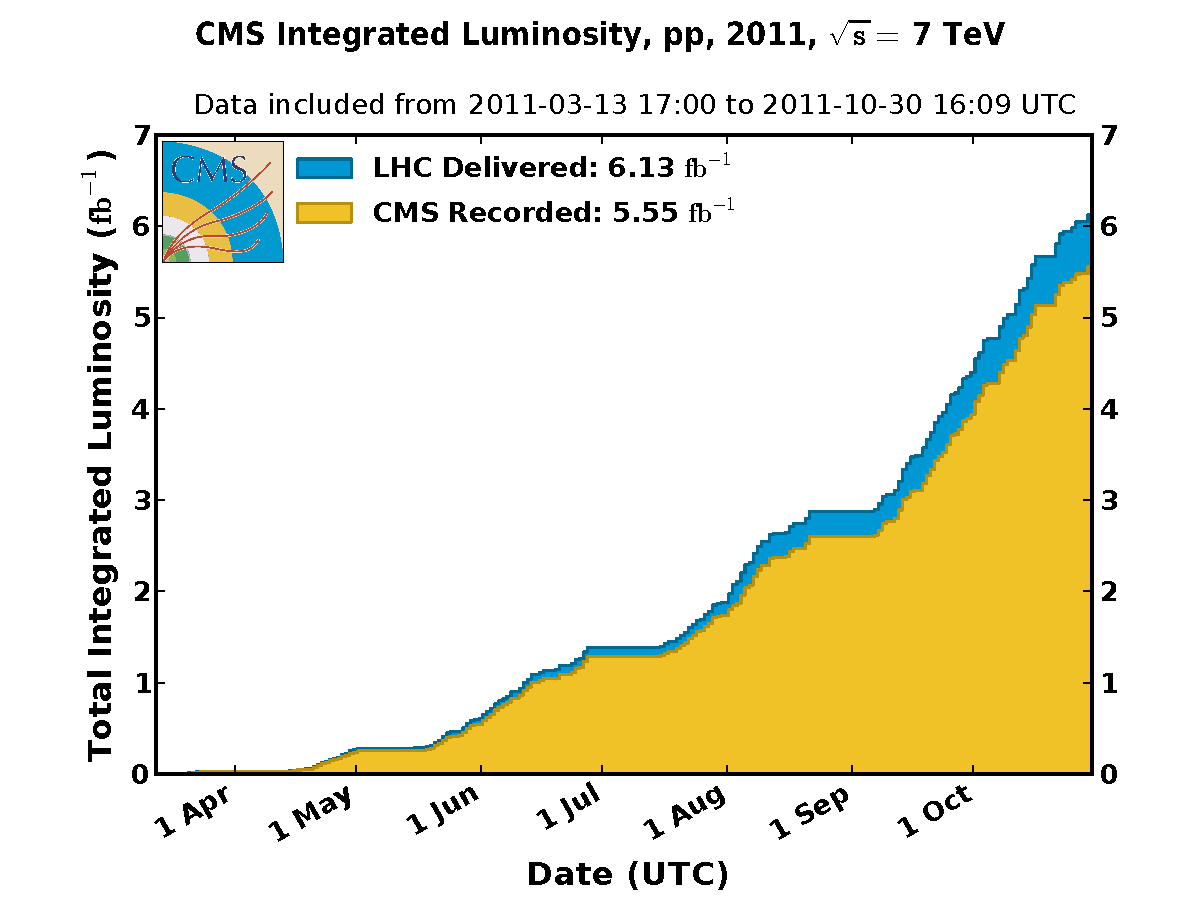
\includegraphics[width=8cm,height=7cm]{ch2/figures/Lumi_pp_2011.pdf}}
 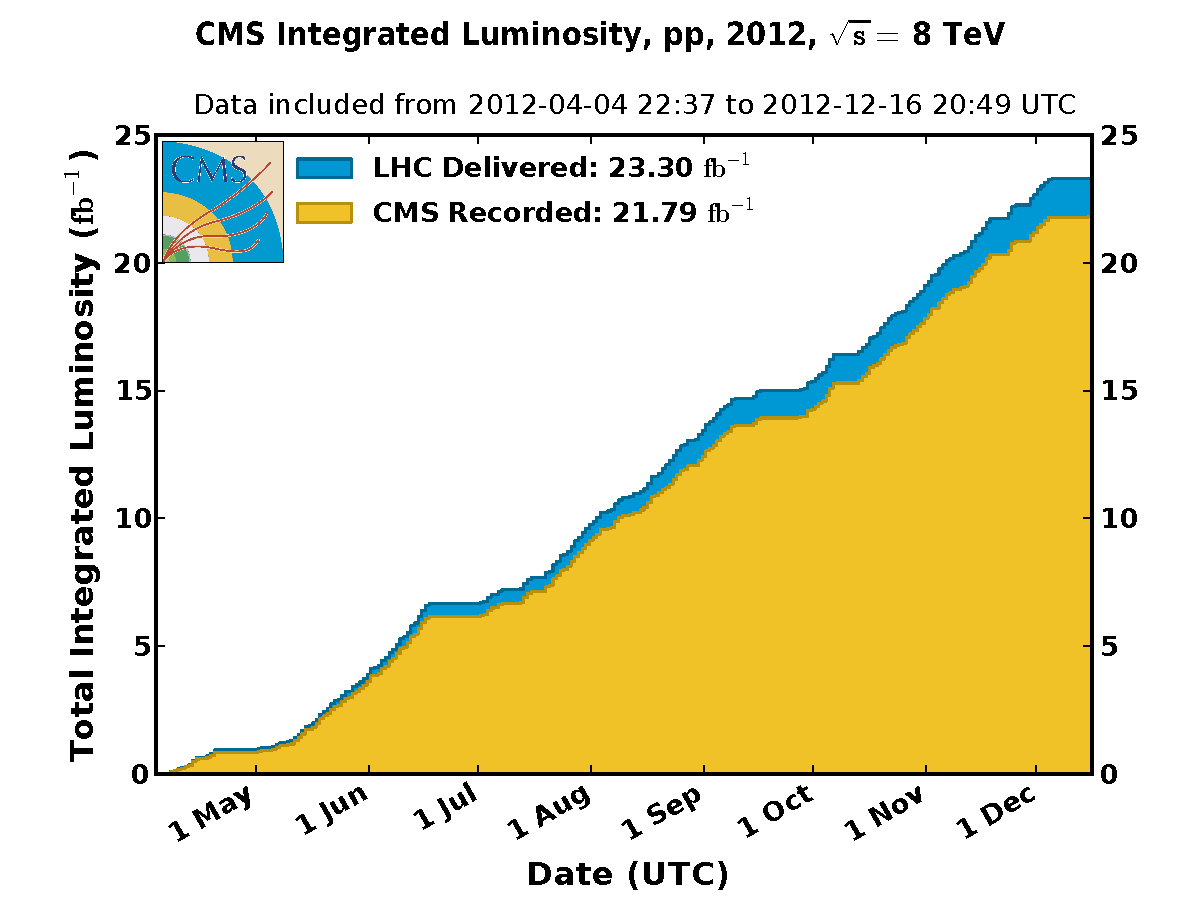
\includegraphics[width=8cm,height=7cm]{ch2/figures/Lumi_pp_2012.pdf}
 \caption{Total integrated luminosity delivered to the CMS experiment for \pp collisions by the LHC during the 2012 run at \sqrteighttev$\,$~\cite{Web:CMSLumi}.}
\label{fig:CMSLumi}
\end{figure}
\section{The Compact Muon Solenoid}
The Compact Muon Solenoid (CMS) experiment~\cite{Chatrchyan:2008aa} consists of a multi purpose $4\pi$ steridian detector and is installed at 
point 5 of the LHC ring, near the village Cessy in France. 
%Each part of the name has certain meaning. ``Compact" is used to denote the dimension of the detector, due to the use of heavier iron in the 
%detector for the magnetic field and muon system. The size of the CMS detector, having a diameter of 15\unit{m} and a length of 28.7\unit{m} 
%is much smaller compared to that of ATLAS detector's diameter of 25\unit{m} and 44\unit{m} length. However, the CMS detector weighs 14\unit{kTon}
%compared to ATLAS detector's weight of 7\unit{kTon}. The word ``Muon" is used due to the excellent muon system of the detector. ``Solenoid" is 
%used because of the geometrical shape of its magnetic field. 

As mentioned in the previous section, the LHC is designed to collide proton beams at $\sqrt{s}=14\unit{TeV}$, with an instantaneous luminosity 
of $10^{34}\unit{cm^{-2}s^{-1}}$. The large \pp total cross section, high beam intensity and short bunch spacing pose very challenging
requirements on the detectors in terms of radiation tolerance, high granularity, time-resolution and online data reduction. The conceptual 
design of the CMS detector was geared towards the detection of the SM Higgs boson and search for new particles, which led to excellent 
reconstruction efficiencies and energy resolutions for electrons, muons, photons, and hadrons~\cite{cmsTDR}. The requirements for the CMS detector
to meet the goals of the LHC physics program, coping with the demanding environmental conditions can be summarized as follows:
\begin{itemize}
\item Good identification and momentum resolution of muons over a wide range of momenta in the barrel region ($\abs{\eta}<2.5$), and a good dimuon mass 
resolution ($\sim$ 1\% at $100\unit{GeV/c^{2}}$ ), and the ability to determine the charge of muons with $\pt < 1\unit{TeV/c}$.
\item A tracker system with an excellent charged particle momentum resolution and reconstruction efficiency. The pixel detector is placed close to the 
interaction region for efficient triggering and offline tagging of $\tau$'s and \bjets.
\item An electromagnetic calorimeter with a good energy resolution and a good mass resolution ($\sim$1\% at $100\unit{GeV/c^{2}}$)
for diphoton and dielectron final states. It was also designed to be efficient in $\pi^{0}$ rejection, and isolation of photons and leptons at high 
luminosities.
\item Good \met\footnote{\met is referred to as the missing transverse momentum and is defined in \sectn{~\ref{sec:coord}}} and dijet mass resolution, requiring hadron calorimeters with a hermetic geometric coverage and with fine lateral segmentation.
\end{itemize}

The design of the CMS detector is similar to the structure of an onion. It consists of several layers of detectors, each one specially designed and
optimized to measure and identify different classes of particles. The main feature of the CMS experiment is a 3.8\unit{T} superconducting solenoid
magnet. Within the field volume are the tracker system, electromagnetic calorimeter, and hadronic calorimeter. A muon detection system is placed
outside the field volume of the solenoidal magnetic field embedded inside iron yoke and having return field for muon momentum measurement. 
A schematic view of the detector system is shown in \fig{\ref{fig:cmsDetector}}. In the following sections, the different components of the CMS 
detector are described in detail.

\begin{figure}[h!]
\centering
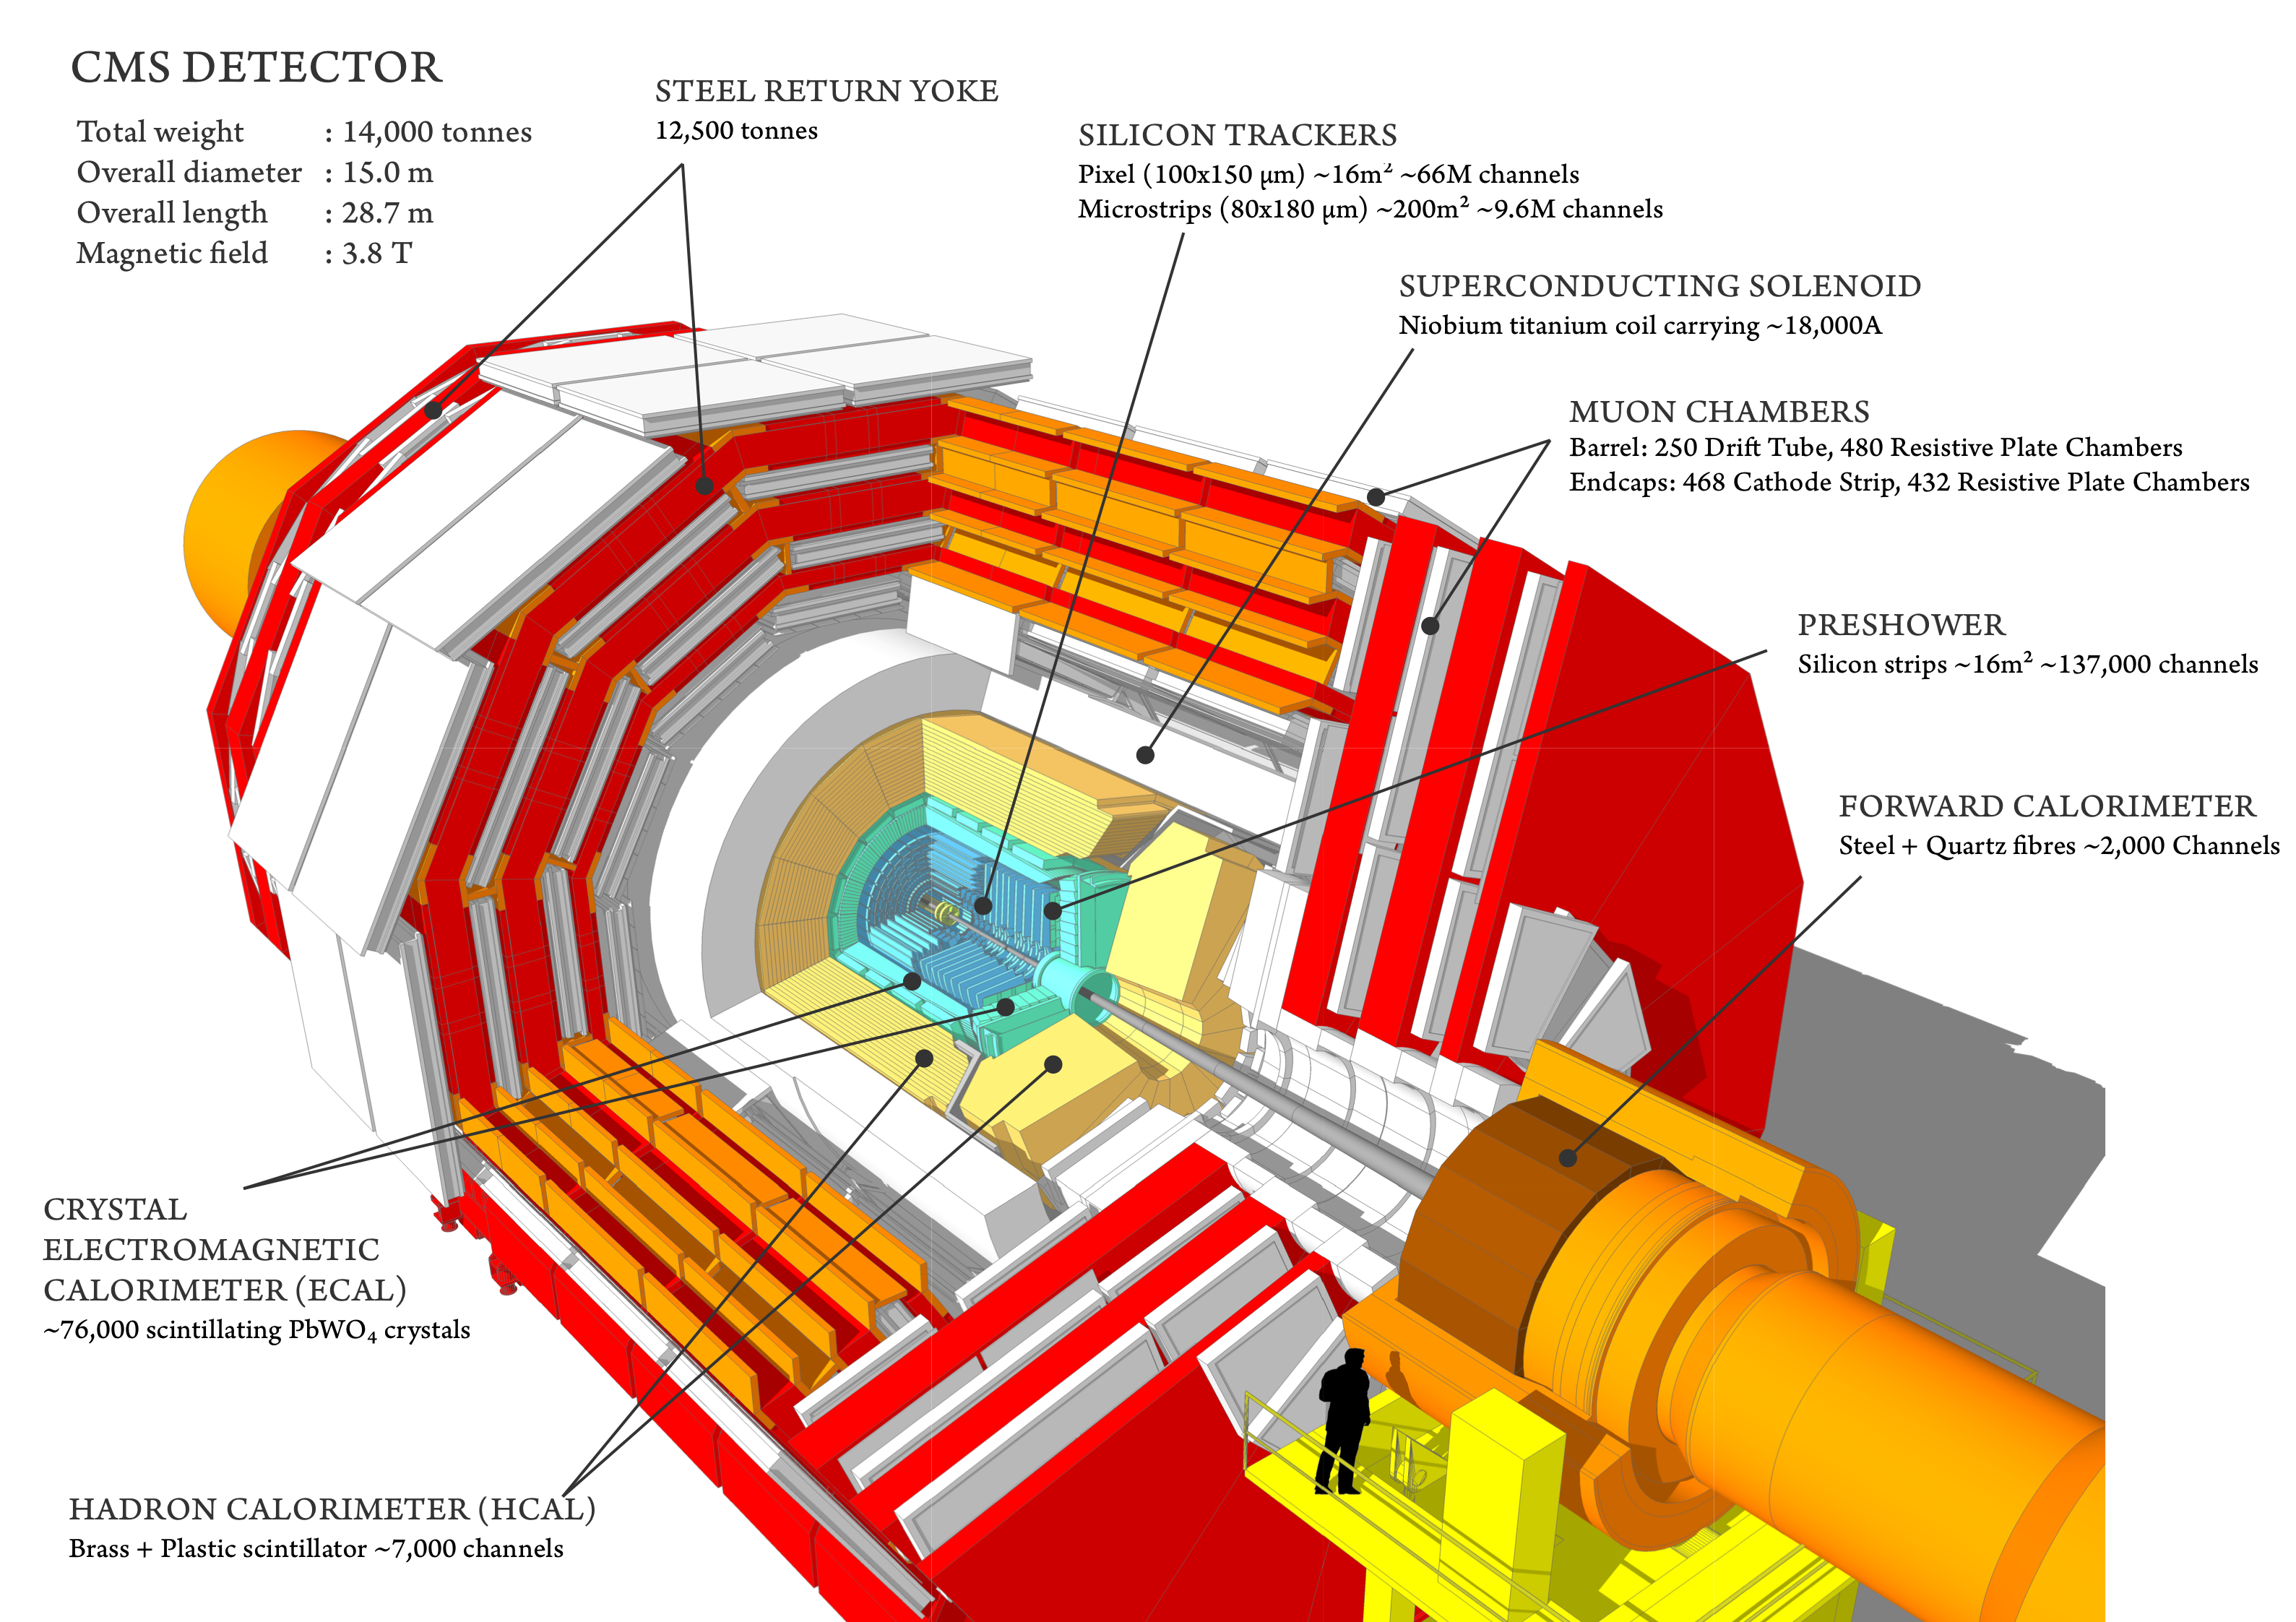
\includegraphics[width=16cm,height=13cm]{ch2/figures/cmsDetector.png}
\caption{Sectional view of the CMS detector~\cite{Web:CERNcds}.}
\label{fig:cmsDetector}
\end{figure}

\subsection{Coordinate System}\label{sec:coord}
The CMS follows a right-handed coordinate system, with origin defined to be the nominal collision point at the center of the detector.
The $x-$axis points radially towards the center of the LHC ring, the $y-$axis vertically upwards while the $z-$axis points west, along the beam
direction towards the Jura Mountains from LHC point 5. The polar angle $\theta$ is measured from the $z-$axis, while the azimuthal angle 
$\phi$ is measured from the $x-$axis in the $x-y$ plane. The radial coordinate, $r$, is defined in the $x-y$ plane. Instead of $\theta$, it is 
often more handy to use rapidity $y$, defined as:
\begin{equation}
y = \frac{1}{2}\ln\left(\frac{E+p_{z}}{E-p_{z}}\right),
\end{equation}
where $E$ and $p_{z}$ are the measured energy and $z-$ component of the momentum carried by the particle. The key reason why rapidity is a crucial 
quantity is because the rapidity differences are invariant with respect to Lorentz boost along the beam axis. But another quantity, known as 
pseudorapidity and defined as:
\begin{equation}
\eta=-ln\left[\mathrm{tan}\left(\frac{\theta}{2}\right)\right],
\end{equation}
is preferred at the hadron colliders. For highly relativistic particles the two quantities are almost identical, $y\simeq\eta$. The rapidity
in terms of pseudorapidity is given by
\begin{equation}
y = ln\left( \frac{\sqrt{m^{2} + \pt^{2}\text{cosh}^{2}\eta} +\pt\text{sinh}\eta}{\sqrt{m^{2} + \pt^{2}}}\right).
\end{equation}
%The only issue with rapidity is that it can be difficult to measure this quantity for highly relativistic particles as it requires both the energy 
%and the total momentum of the particle and in reality it is difficult to get the total momentum of a particle, especially at high values of the 
%rapidity where the $z-$component of the momentum is large, and the beam pipe can be in the way of measuring it precisely. 
The angular separation of two events, ($y_{2}-y_{1}$, $\phi_{2}-\phi_{1}$) is invariant with respect to boosts along the beam axis
and the angular distance between two objects, as observed from the origin of the CMS detector, is expressed as:
\begin{equation}
R = \sqrt{(\deta)^{2}+(\dphi)^{2}}.
\end{equation}
In collider experiments, the incoming particles collide head-on and have no transverse momentum before scattering and therefore by momemtum 
conservation, the final state particles must have zero total transverse momentum. Hence, the momentum and energy of the object are measured 
transverse to the beam direction, denoted by \pt and \et, respectively, where $\pt = \sqrt{p_{x}^{2} + p_{y}^{2}}$ and $\et = E\,\text{Sin}\theta$.
The missing transverse momentum is defined as the negative vector sum of all particles detected by the detector, $\metVec\equiv -\sum \vec{\pt}$.
Momentum conservation dictates that \metVec is equal, in the limit of a perfect detector efficiency and resolution, to the vector sum of transverse 
momentum of all undetected particles such as neutrinos or some new particle and the energy lost in nuclear processes.

\subsection{Magnet}
The choice of the magnet is crucial for ensuring good performance for a high energy physics experiment. Precise measurement of the charged
particle momenta at a wide range of energies requires high bending power that can be achieved using strong magnetic field. For a charged
particle in a uniform magnetic field, B, the momentum of the particle is given by, $p=\gamma{mv}=qBr$, where $q$ is its charge, $m$ is its
mass and $r$ is the bending radius of the particle. The trajectory of a charged particle in the magnetic field is an arc of radius $r$ and path 
length $L$. The sagitta of the trajectory, defined as the perpendicular distance from the midpoint of the arc's chord to the arc itself and is given 
by $s = \frac{L^{2}}{8r} = \frac{qBL^{2}}{8p}$. Assuming that the particle crosses the full solenoid, $L$ is equal to the radius of the solenoid.
The \pt resolution depends on the magnetic field and solenoid radius as, $\frac{dp}{p}\propto\frac{p}{BL^{2}}$.

Therefore, for improvement in the resolution both a large size and a strong magnetic field is needed. The CMS design~\cite{cmsMagnet} having a 
solenoid of 6\unit{m} in diameter (and also a large tracker that defines the measurable path length) and a strong magnetic field of 3.8\unit{T} meets 
the requirement.

The CMS magnet~\cite{cmsMagnet} consists of two main parts, the coil and the yoke. The coil forms the superconducting solenoid which utilizes a 
4-layer winding made from a stabilized reinforced NbTi conductor to give a magnetic field of 3.8\unit{T}. The yoke comprised of 11 large elements, 
5 barrel wheels and 6 endcap disks, that returns magnetic flux yielding a field of about 2\unit{T}. The yoke was designed to achieve a balance
between the outer diameter of the yoke and the size of the muon system\footnote{Muon system is described in more detail in \sectn{\ref{sec:muon}}}~\cite{Chatrchyan:2008aa}. At full current, the energy stored in the
magnetic field is $\sim2.7\unit{GJ}$.

\subsection{Tracking System}
The tracker is the innermost sub-system of the CMS detector. It is designed to measure precisely and efficiently the trajectories of charged 
particles from the interaction point, and reconstruct both primary and secondary vertices. It not only reconstructs the paths of muons, 
electrons, and charged hadrons, but also the tracks coming from the decay of very short-lived particles such as $b-$ and $c-$quarks, with high momentum resolution and efficiency.
\begin{figure}[h!]
\centering
%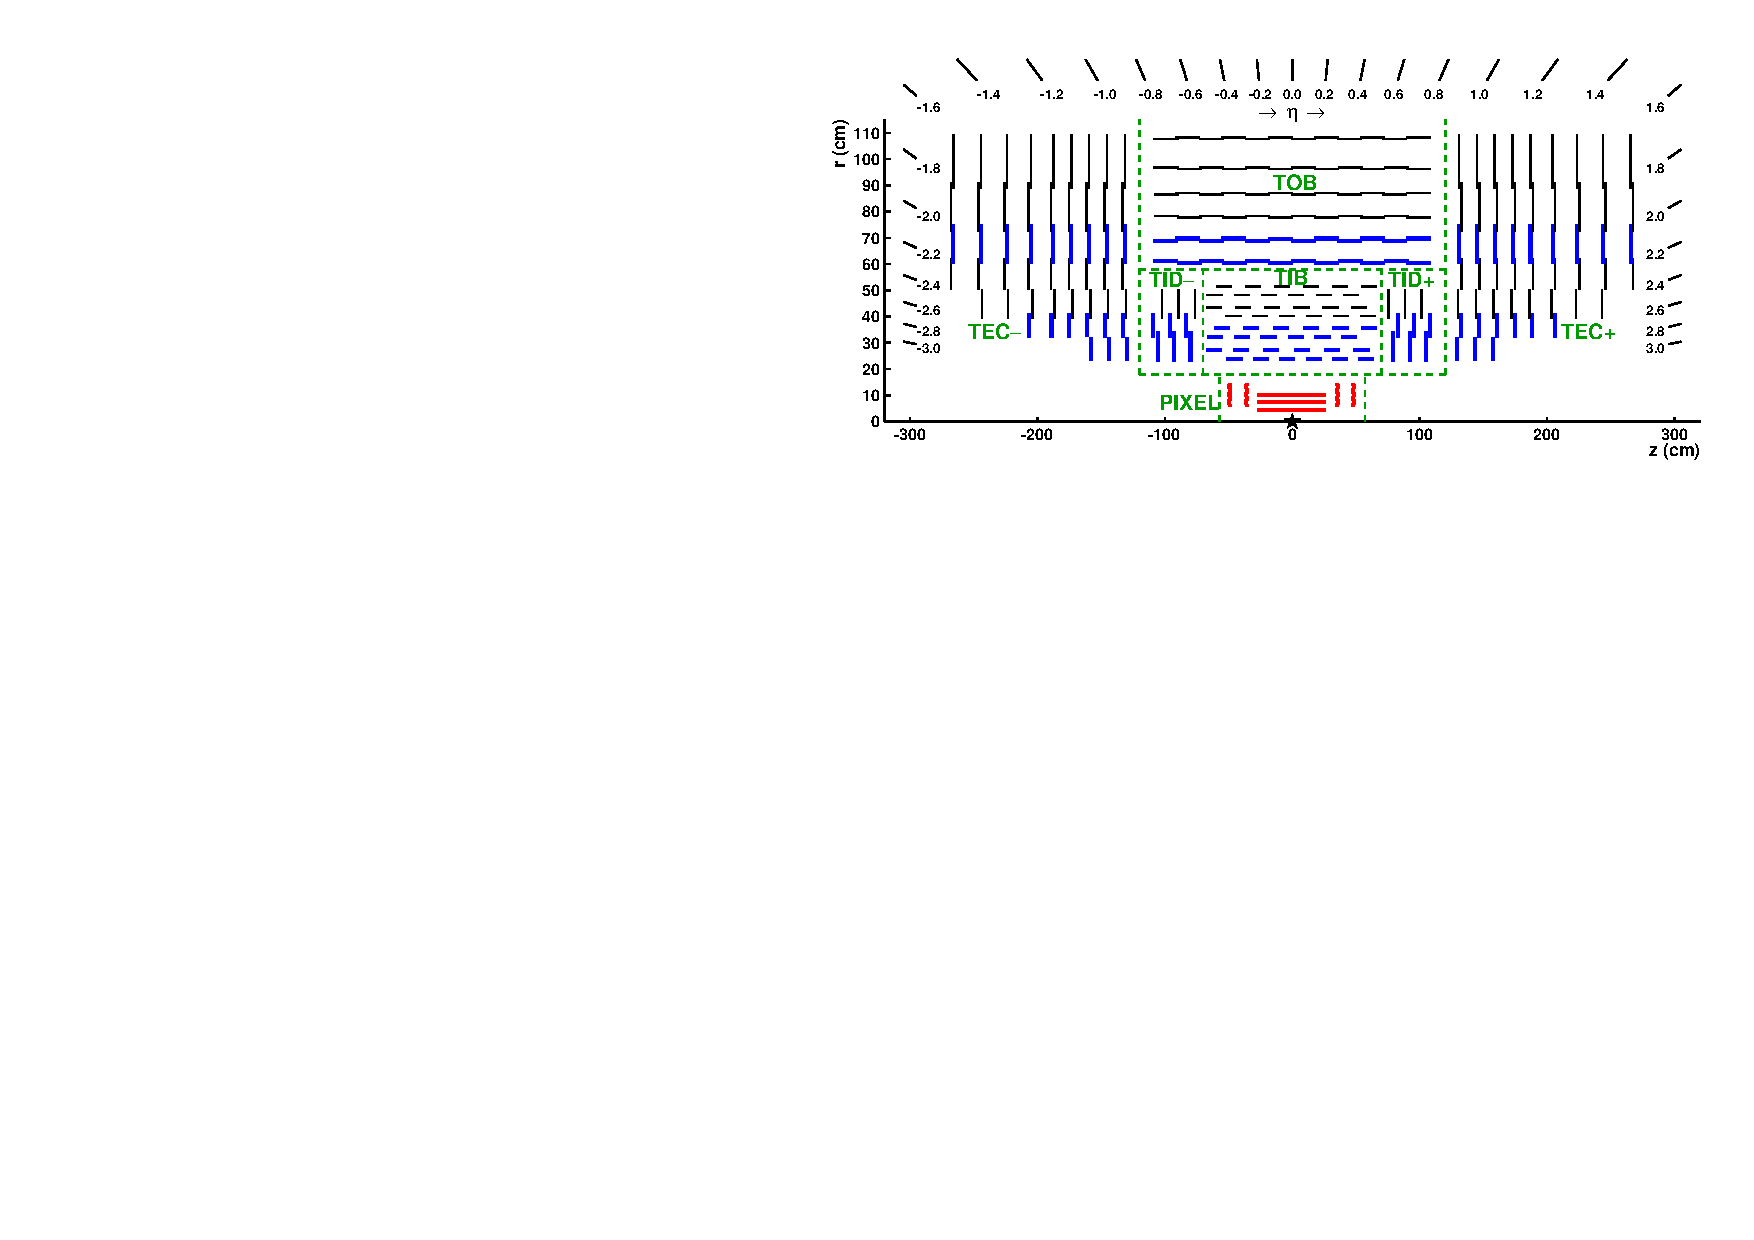
\includegraphics[width=14cm,height=7cm]{ch2/figures/TrackerLayoutNew.pdf}
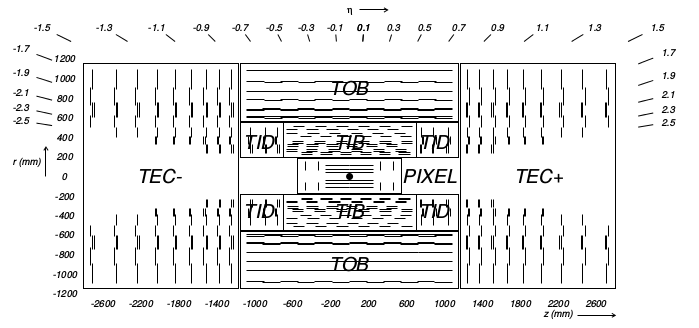
\includegraphics[width=14cm,height=7cm]{ch2/figures/TrackerLayout.png}
\caption{ Schematic view of the CMS tracker in the $r-z$ plane~\cite{Chatrchyan:2008aa}. Each line depicts a detector module and double lines represents back-to-back modules. Abbreviations TEC, TIB, TID, TOB, etc. are described later in text.}
\label{fig:trackerLayout}
\end{figure}

A tracker system~\cite{Chatrchyan:2008aa,Karimaki:368412} covering the region $\abs{\eta}<2.5$ and employing more than 200\unit{m^2} of active Si 
sensors is shown in \fig{\ref{fig:trackerLayout}}. It surrounds the interaction point and has a length of 5.8\unit{m} and a diameter of 2.5\unit{m}. 
The CMS solenoid provides a homogeneous magnetic field of 3.8\unit{T} over the full volume of the tracker. At high luminosity, 20 overlapping \pp 
collisions at the LHC would, on an average, result in 1000 particles traversing the tracker for every bunch crossing, \ie every 25\unit{ns}. Therefore, 
a detector featuring high granularity and fast response is needed to cope with the large levels of occupancy and radiation. In addition, the intense 
particle flux will also cause severe radiation damage to the tracking system. These requirements on granularity, speed and radiation hardness 
necessitate a tracker design based entirely on silicon detector technology.

The tracks in the CMS are seeded by the hits in the tracker detector. The compatible hits are added to update the trajectory 
until either the detector boundary is reached, or no additional compatible hits\footnote{Hits compatible with the extrapolation of parameters
for a track, growing trajectory of a track, and their covariance matrix in the detector material.} can be found. The collection of hits is then
used to obtain the best estimate of the track parameters. However, the large amount of material within the tracker volume affects the overall
event topology and reconstruction due to electron bremsstrahlung, conversions of photons to electron pairs and nuclear interactions.
Therefore, it is important to estimate the amount of material of the CMS tracker. This is shown in \fig{\ref{fig:MaterialBudget}} --- both in 
%\fig{\ref{fig:MaterialBudget}} is taken from link~\cite{Chatrchyan:2014fea}
\begin{figure}[h!]
\centering
 \subfloat[]{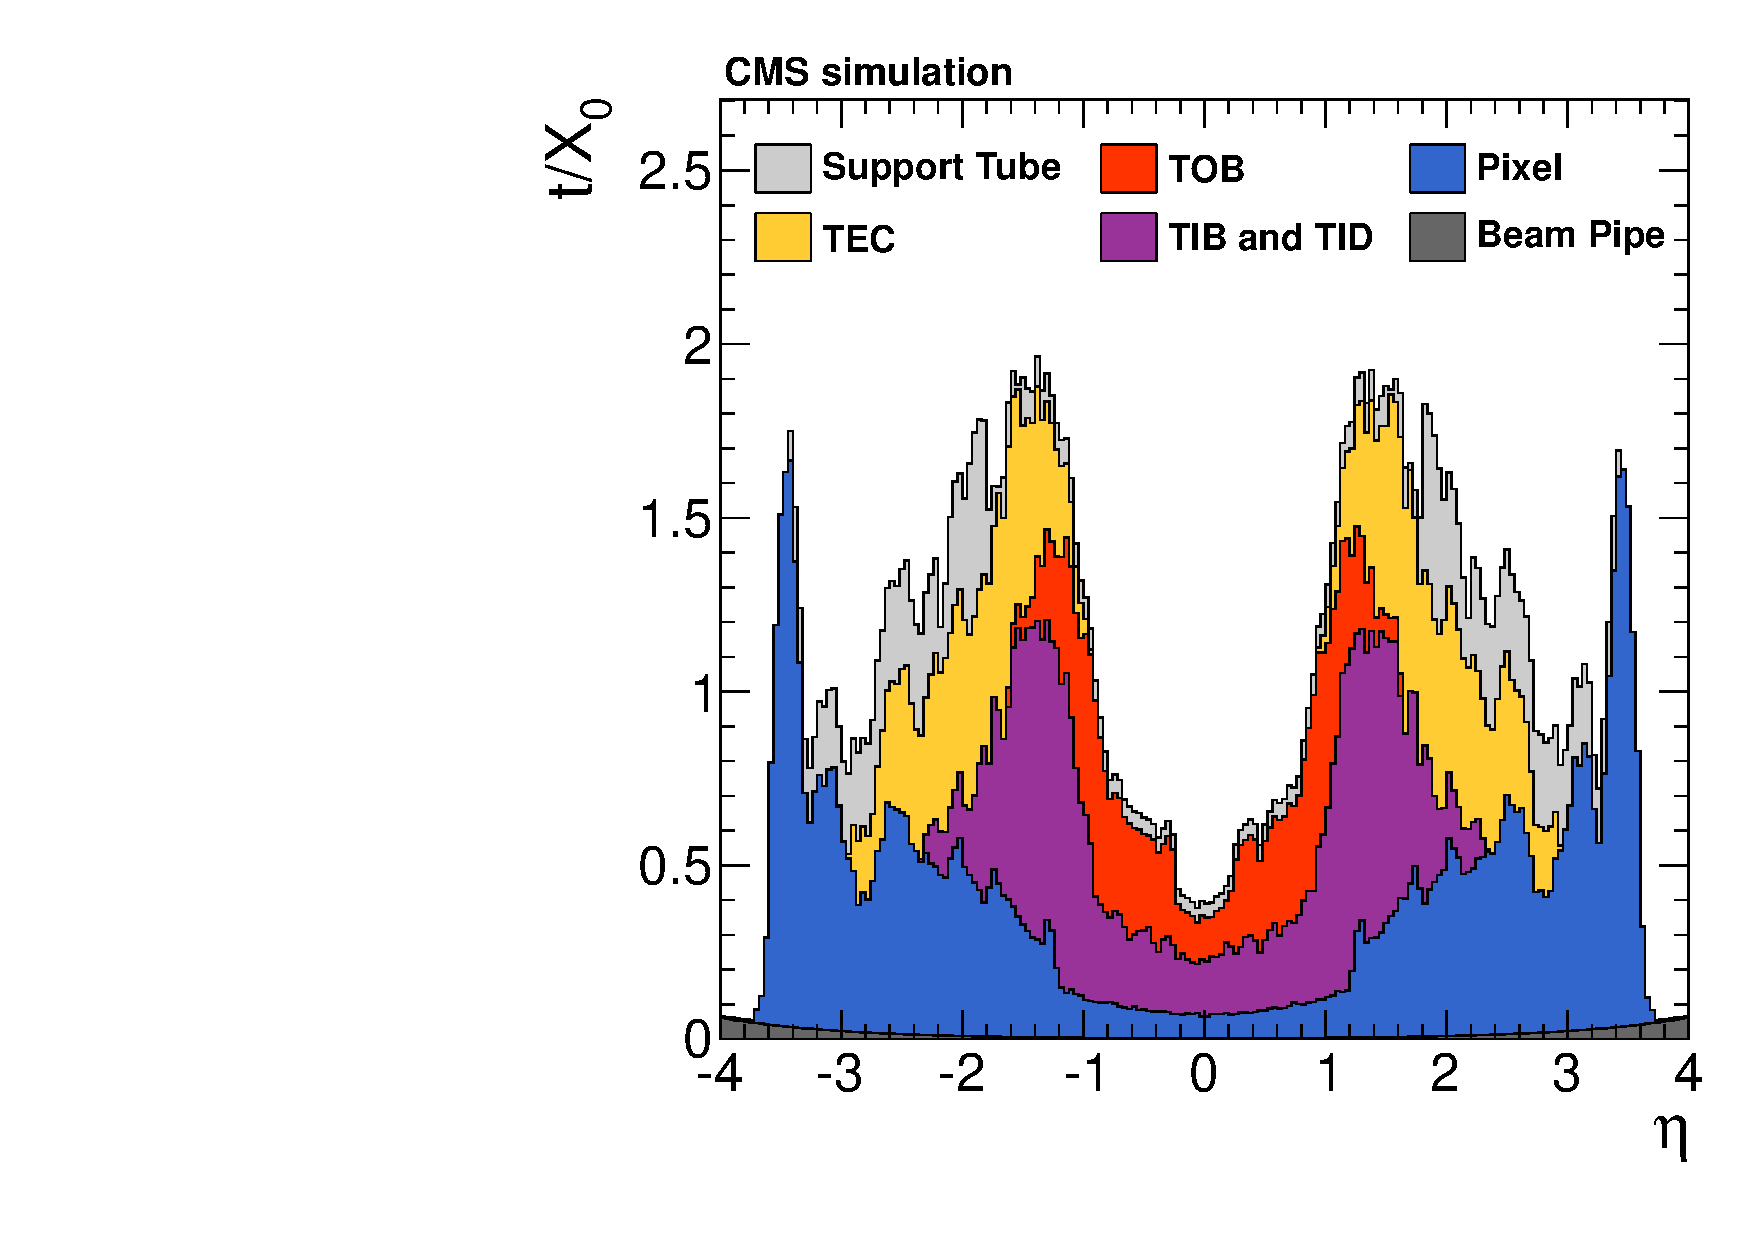
\includegraphics[width=7.6cm,height=7cm]{ch2/figures/MaterialBudget_RadLengths.pdf}}
\hspace{0.5cm}
 \subfloat[]{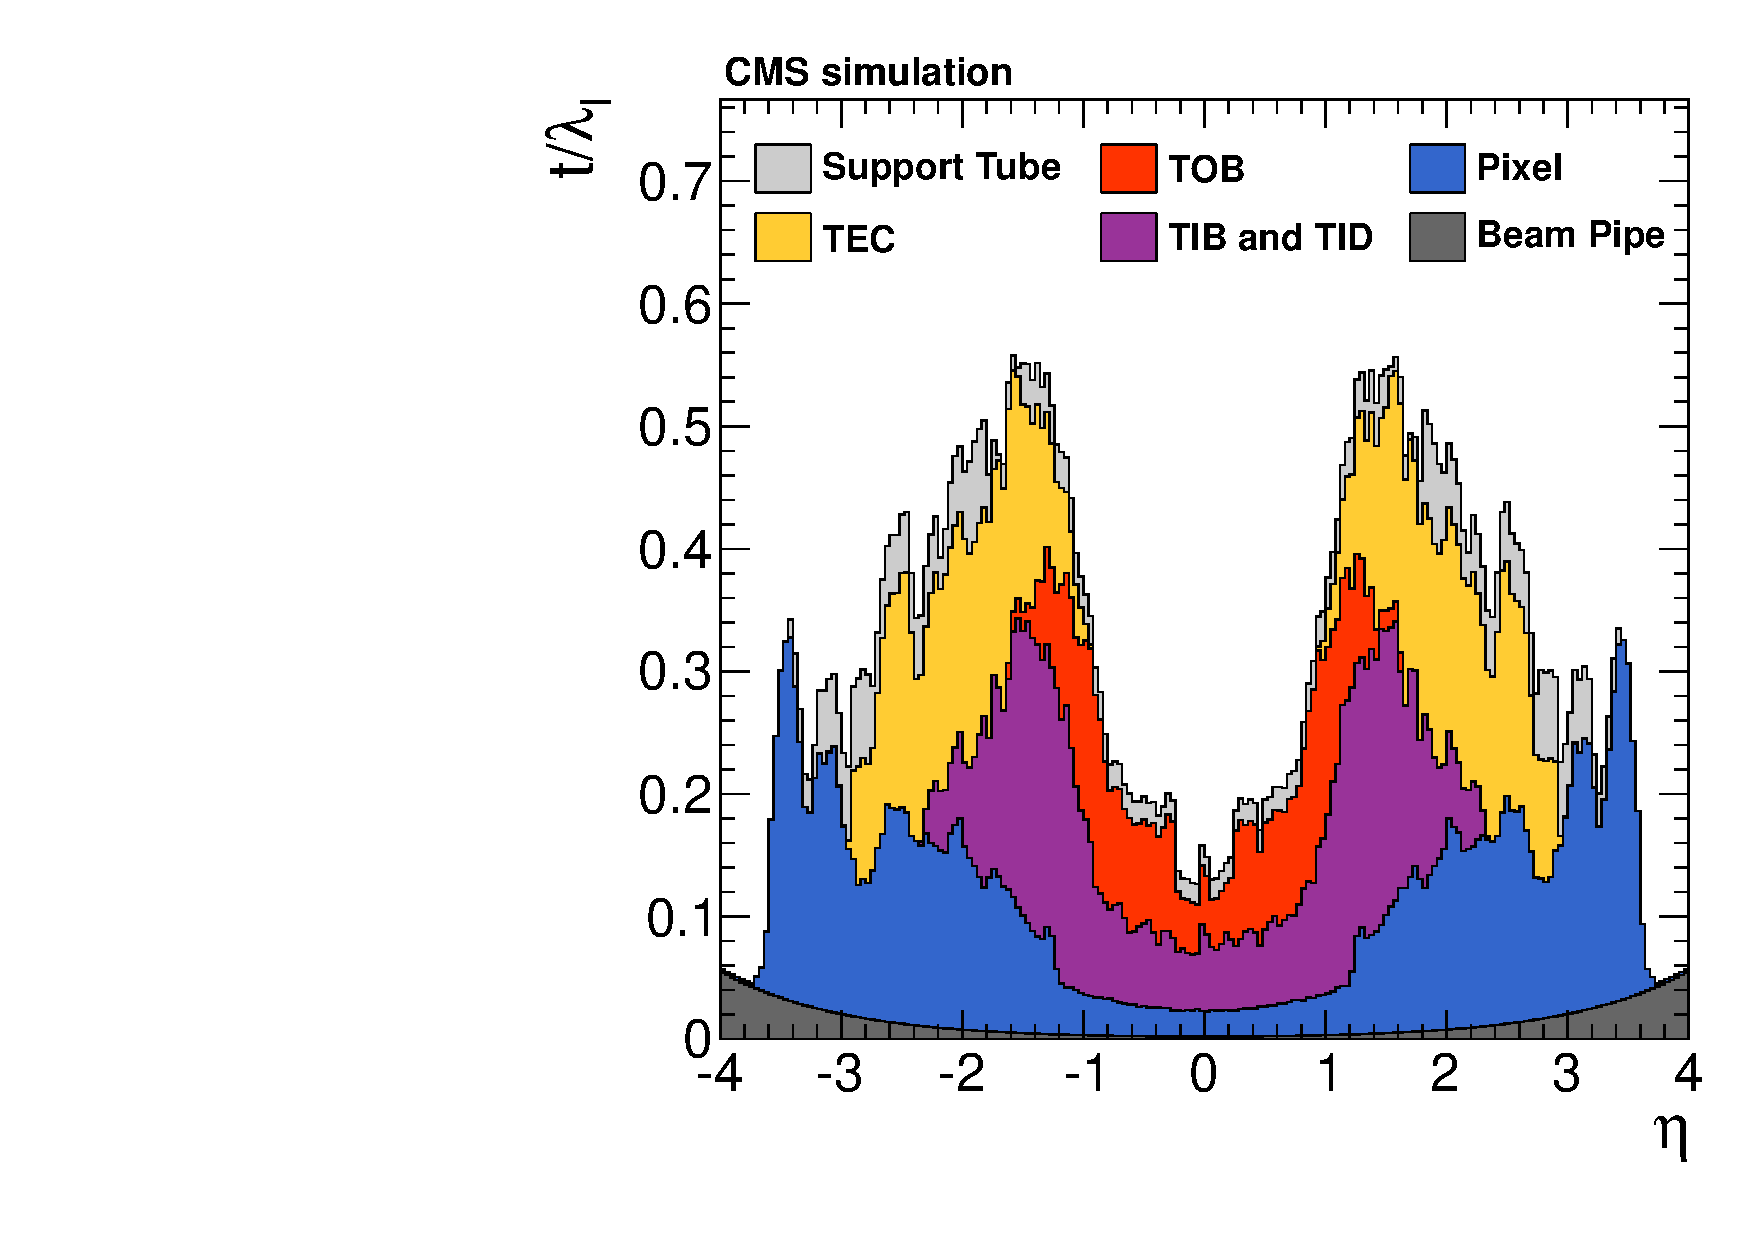
\includegraphics[width=7.6cm,height=7cm]{ch2/figures/MaterialBudget_InteractionLengths.pdf}} 
 \caption{Total thickness of the tracker material traversed by a particle produced at the nominal interaction point, as a function of pseudorapidity, expressed in units of (a) radiation length $\mathrm{X_0}$ and (b) nuclear interaction length $\lambda_I$~\cite{Chatrchyan:2014fea}.}
\label{fig:MaterialBudget}
\end{figure}
units of radiation length ($\mathrm{X_0}$) and nuclear interaction length ($\lambda_I$) as a function of pseudorapidity, as estimated from simulation 
within about$\sim10\%$ accuracy~\cite{Karimaki:368412,CMS:2010nua,Chatrchyan:2014fea}. The $\mathrm{X_0}$ corresponds to the mean distance over 
which an electron loses a fraction 1/e of its energy. It also corresponds to 7/9 of the mean free path for pair production of a photon. At $\eta=0$, 
the tracker material budget corresponds to about 0.4\unit{X_0}, while at the boundary between the barrel and the endcaps, the material budget reaches 
a value of 1.8\unit{X_0} due to cabling and other services like mechanical support in this region. The CMS tracker is composed of a pixel detector 
and a silicon strip tracker which are described in details in the sections to follow. 

\subsubsection{Pixel Detector}
The pixel detector~\cite{Chatrchyan:2008aa,Karimaki:368412} is the part of the tracking system closest to the interaction region with a
 pseudorapidity coverage of $\abs{\eta}<2.5$, as shown in \fig{\ref{fig:pixelDetector}}. Being very close to the interaction 
vertex and beam direction, it is inundated with a very large particle flux. It contains about 66\unit{million} Si pixels, allowing it to provide 
precise and highly accurate tracking points in three dimensional space, ($r$, $\phi$ and $z$) for all emerging particles. This is essential for 
reconstruction of secondary vertex from decays of \bquark and tau leptons and forming seed tracks for the reconstruction of outer tracks. The pixel 
cells, of size 100$\times$150\unit{\mu{m}^{2}}, are used to attain an occupancy level of $\sim 10^{-1}$/(pixel$\times$bunch-crossing). 
The pixel has a zero-suppressed analog pulse height read-out scheme that improves position resolution and helps in separating signal from noise hits 
as well as identifying large hit clusters from overlapping tracks. 
\begin{figure}[h!]
\centering
 \subfloat[]{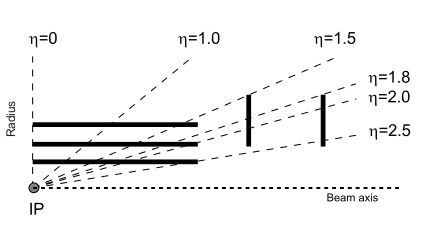
\includegraphics[width=6cm,height=5cm]{ch2/figures/PixelLayout.png}}
\hspace{1cm}
 \subfloat[]{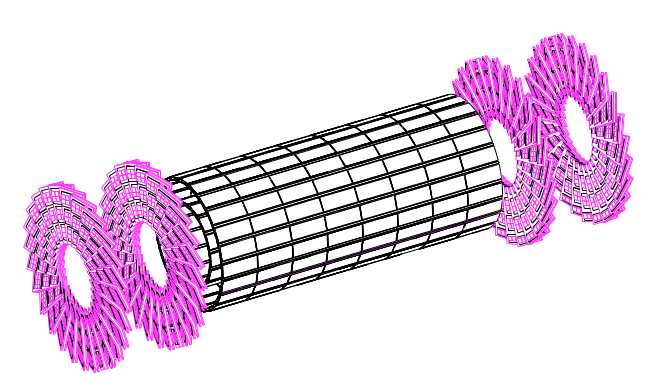
\includegraphics[width=7cm,height=6cm]{ch2/figures/pixelDetector.png}} 
 \caption{(a) Hit coverage and (b) geometrical layout of the CMS pixel detector~\cite{Chatrchyan:2008aa}.}
\label{fig:pixelDetector}
\end{figure}

The layout of the pixel system consists of three barrel layers (\gls{BPIX}) with two endcap disks (\gls{FPIX}). The 53\unit{cm} long BPIX 
layers are located at mean radii of 4.4, 7.3 and 10.2\unit{cm}, whereas the FPIX extends from 6 to 15\unit{cm} in radius and are placed at 34.5 and 
46.5\unit{cm} on both sides of the nominal interaction point. The BPIX (FPIX) layers contain 48\unit{million} (18\unit{million}) pixels covering a 
total area of 0.78 (0.28)\unit{m^2}. The forward detectors are tilted at 20$^{\circ}$ in a turbine-like geometry to induce charge 
sharing~\cite{Atac:2002mk}. The pixel detector has a spatial resolution in the range of $15-20\unit{\mu{m}}$~\cite{Karimaki:368412}.
Unfortunately, they would need to be replaced during the time period of the experiment, due to radiation damage.



\subsubsection{Silicon Strip Detectors}
The silicon strip tracker~\cite{Chatrchyan:2008aa,Karimaki:368412} is composed of 15148 detector modules distributed among the four different 
subsystems $-$ Tracker Inner Barrels (\gls{TIB}), Tracker Inner Disks (\gls{TID}), Tracker Outer Barrels (\gls{TOB}) and Tracker EndCaps (\gls{TEC}). Each module
carries either one thin (320\unit{\mu{m}}) or two thick (500\unit{\mu{m}}) silicon sensors. The dimension of the strips increases with increasing 
distance from the interaction point so that the occupancy level is kept to $\sim1\%$. The occupancy is defined as the number of strip measurements 
in an event divided by the number of all active strips. The silicon detectors work in much the same way as the pixels $-$ a charged particle crosses 
the material, knocks out electrons from the atom and within the applied electric field, gives a very small pulse of current lasting a few nanoseconds. 
The schematic longitudinal view of the silicon strips in terms of different layers and their arrangements in $\eta$ and $z$ plane is shown in 
\fig{\ref{fig:SiliconStrips}} .
\begin{figure}[h!]
 \centering
 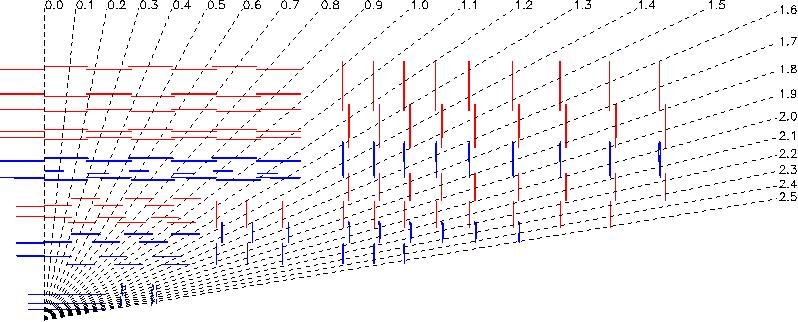
\includegraphics[width=12cm,height=6cm]{ch2/figures/SiliconStrip.png}
 \caption{A Schematic layout of the silicon microstrip detector~\cite{Chatrchyan:2008aa}.}
 \label{fig:SiliconStrips}
\end{figure}

The TIB and TID are composed of four barrel layers and three disks at each end. The silicon strip tracker provides up to four $r-\phi$ measurements 
with a position resolution of 23\unit{\mu{m}} in the two inner layers and 35\unit{\mu{m}} in the two outer layers~\cite{Chatrchyan:2008aa}. The TIB 
and TID are surrounded by the six layers of TOB, providing a resolution of 53\unit{\mu{m}} in the first four layers and 35\unit{\mu{m}} for the outer 
two layers~\cite{Chatrchyan:2008aa}. Beyond $z=118\unit{cm}$ TEC provides additional forward coverage up to $\abs{\eta}<2.5$, giving nine $\phi$ 
measurements per trajectory and extending up to 282\unit{cm}~\cite{Chatrchyan:2008aa}.

\subsection{Calorimeter System}
A calorimeter is a detector which measures the energy of a particle. The CMS calorimeters are designed to measure the energy of electrons, photons 
and hadrons (jets) produced in collisions. The CMS calorimeter is divided into electromagnetic and hadronic sections. The electromagnetic calorimeter 
(\gls{ECAL}) is used to measure the energy of particles which interact electromagnetically such as photons and electrons whereas the hadronic calorimeter 
(\gls{HCAL}) is designed to measure the energy of strongly interacting particles. Hadrons interact via strong force leading to showers that has both 
electromagnetic and hadronic component. The hadronic component of the shower scales with the nuclear interaction length and can not be contained 
within the ECAL. Muons, though interact via electromagnetic force, behave in a very different way. They loose energy primarily through ionization,
with energy losses of the order of $1-2$\unit{MeV/g/cm^{2}} and, therefore, different sub-system is needed for the detection of muons. 
Interacting with matter via the weak force, neutrinos typically pass through the matter unimpeded and undetected, and can be observed only indirectly 
as an imbalance in event energy in the transverse plane. The measurement of this imbalance, termed as missing transverse energy, plays a critical 
role for new physics searches, such as compositeness, supersymmetry, extra dimensions etc.

\subsubsection{Electromagnetic Calorimeter}
The ECAL~\cite{Chatrchyan:2008aa,ecalTDR} is a homogeneous, hermetic calorimeter made up of 61200 lead tungstate (PbWO$_4$) scintillating crystals 
mounted in the central barrel part, accompanied by 7324 crystals in each of the two endcaps. It covers the pseudorapidity region up to
$\abs{\eta}<3$, and is complemented, in the forward region ($1.653<\abs{\eta}<3.0$) by Si-Pb preshower, as shown in \fig{\ref{fig:Ecal}}. In order 
to fulfill the scientific goals of the CMS, the ECAL was designed to have a high energy resolution for e/$\gamma$ objects. To achieve this, the ECAL 
was positioned inside the CMS magnet so that the amount of energy loss due to the material upstream can be minimized. 
\begin{figure}[h!]
 \centering
 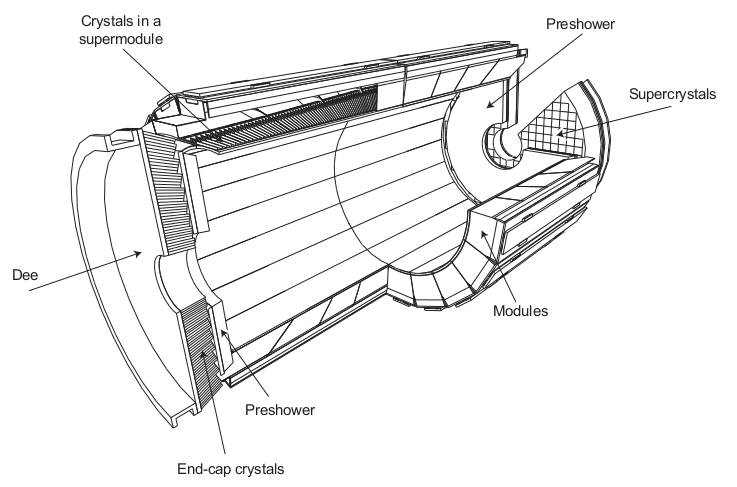
\includegraphics[width=13cm,height=8cm]{ch2/figures/cmsECAL.png}
 \caption{A schematic design of the CMS ECAL showing the arrangement of crystals, supermodules and endcaps with the preshower in front~\cite{Chatrchyan:2008aa}.}
 \label{fig:Ecal}
\end{figure}
Within the LHC environment, it is important to design a calorimeter which is fast, has fine granularity and is radiation tolerant. 
The PbWO$_4$ crystals have a large density (8.28\unit{g}/cm$^{3}$), a small radiation length X$_{0}$ (0.89\unit{cm}), and a small Moli\'{e}re 
radius (2.2\unit{cm}), which makes them an appropriate choice for a compact and high granular calorimeter. The total amount of material between the 
interaction point and the ECAL increases from 0.4\unit{X_0} close to $\eta=0$ to almost 2\unit{X_0} near $\abs{\eta}=1.4$, before falling 
again to about 1.3\unit{X_0} around $\abs{\eta}=2.5$. Therefore, the resolution of the ECAL depends on the \pt and $\eta$ of the object,
and whether the electron or photon undergoes bremsstrahlung.

The ECAL barrel (\gls{EB}) covers the region $\abs{\eta}<1.48$, and has an internal surface radius of 1290\unit{mm}. It is made up of 61,200 
trapezoidal crystals. Each crystal has a frontal area of approximately $22\times22\unit{mm^{2}}$ and a length of 230\unit{mm} (25.8\unit{X_{0}}),
which leads to a granularity of 0.0174 in $\eta$ and $\phi$. A half-barrel consist of 18 supermodules, each containing 1700 crystals and covering
$20^{\circ}$ in $\phi$. Photodetectors are placed in front of the crystals to collect the light and convert it into signals which can be read out 
by the electronics chain. Since the light yield from the PbWO$_{4}$ crystals is relatively low, amplification of the signal needs to be done, and 
hence silicon avalanche photodiodes (\gls{APDs}) are used. In addition to intrinsic gain, APDs are also insensitive to magnetic fields and have high 
radiation resistance and are, thus, suitable for EB.

The endcaps (\gls{EE}) cover the region $1.48<\abs{\eta}<3.00$, are located at $\abs{z}>3154\unit{mm}$ and are composed of 4 half disks. Each half-disk 
is made up of 3,662 trapezoidal crystals each having a frontal area of $28.6\times28.6\unit{mm^{2}}$ and a length of 220\unit{mm} 
(24.7\unit{X_{0}}). The crystals in each disk are organized into 138 standard $5\times5$ supercrystal units with 52\unit{mm} wide voids in between 
the groups. The crystals are arranged in a quasi-projective geometry pointing $\pm1300\unit{mm}$ beyond the nominal  interaction point. 
Photodetectors used in the EE are Vacuum phototriodes (\gls{VPTs}). The VPTs can be operated in a very high radiation environment and hence are used in the EE.

A preshower detector is a pair of sampling calorimeters designed to distinguish neutral pions from real photons and improves the position
measurement of electrons and photons with high granularity. Each calorimeter consists of two planes of silicon sensors interleaved with 
a total of 3\unit{X_{0}} of lead and is located in front of the EE and covers the region $1.65<\abs{\eta}<2.60$.

The ECAL energy resolution for electromagnetic showers below 500\unit{GeV}, can be parametrized as :
\begin{equation}
\left(\frac{\sigma}{E}\right)^{2} = \left(\frac{S}{\sqrt{E}}\right)^{2} + \left(\frac{N}{E}\right)^{2} + C
\end{equation}
where $S$ is the intrinsic stochastic term, $N$ is the noise term and $C$ is the constant term with details as follows :
\begin{itemize}
\item Stochastic term ($S$) : This includes contribution from event-to-event fluctuation in the lateral shower containment, photostatistics
contribution, fluctuations in the energy deposited in the preshower absorber (where present) with respect to what is measured in the 
preshower silicon detector. The contribution of these fluctuations to the energy resolution of the calorimeters follow Poissonian distribution,
hence the resolution scales as $1/\sqrt{E}$.
\item Noise term ($N$) : The three contributions to the noise term include : electronics noise; digitization noise; and pileup noise. The signal 
amplitude in the test beam is reconstructed using a simple digital filter. The noise measured, after this amplitude reconstruction, for 
channels in barrel supermodules is $\sim40\unit{MeV}$/channel in the highest gain range. This noise includes both electronics and 
digitization noise and varies as $1/E$. The noise from the pileup is found to be very small.
\item Constant term ($C$): The most important contributions to the constant term include: non-uniformity of the longitudinal light collection,
 inter calibration errors, and leakage of energy from the back of the crystal. %The constant term can be reduced by utilizing radiation hard media and
% performing in-situ calibration. The CMS calorimeter accounts for both the factors by utilizing a laser monitoring and a calibration system
\end{itemize}
The test beam results~\cite{Chatrchyan:2008aa,CMS:2010zta} using the energy measurement in $3\times3$ crystal lattice, lead to the following values 
for the various terms : $S=2.8\%$, $N=124\unit{MeV}$, and $C=0.3\%$ in the barrel regions and $S=5\%$, $N=500\unit{MeV}$ and $C=0.3\%$ for the 
endcap regions.

\subsubsection{Hadronic Calorimeter}
The hadronic calorimeter~\cite{Chatrchyan:2008aa,hcalTDR} is a sampling calorimeter surrounding the ECAL, which is used in conjunction with 
the ECAL to measure the energy and direction of hadronic particles and to estimate the missing transverse momentum (\met).
%The determination of missing energy and jets are crucial for new particles and phenomena, such as supersymmetric partners of 
%quarks and gluons. Indirectly, the HCAL also helps in the identification of electrons and photons. 
The HCAL is composed of four sub-detectors $-$ HCAL Barrel (\gls{HB})~\cite{Abdullin:2008zzb}, HCAL Endcaps (\gls{HE})~\cite{Baiatian:2008zz}, 
HCAL Outer (\gls{HO})~\cite{Abdullin:2008zza}, and HCAL Forward (\gls{HF})~\cite{Bayatian:2006jz} as shown in \fig{\ref{fig:cmsHCAL}}. 
The HCAL consists of plastic scintillator tiles read out with embedded wavelength-shifting (\gls{WLS}) fibres interleaved with overlapping brass plates 
for the absorber material.
\begin{figure}[h!]
 \centering
 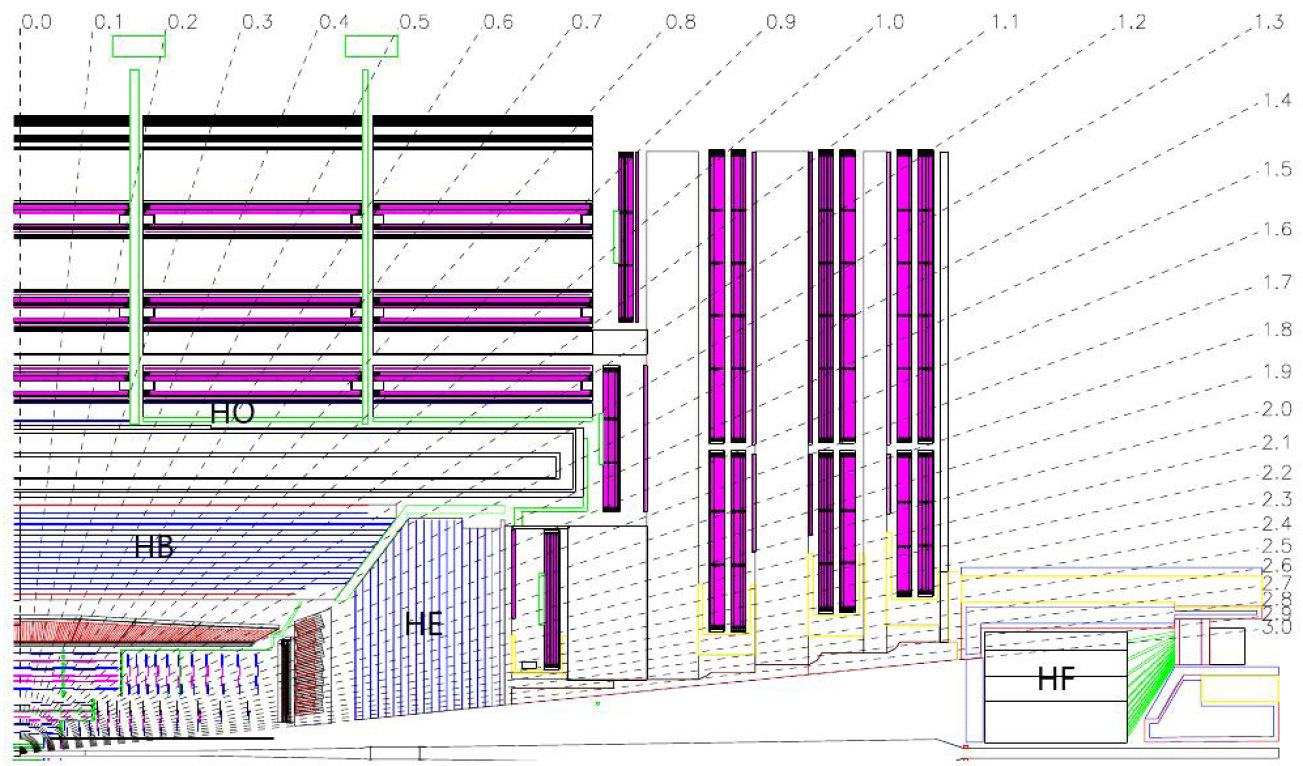
\includegraphics[width=13cm,height=8cm]{ch2/figures/cmsHCAL.png}
 \caption{A schematic design of the CMS HCAL showing the barrel section (HB), endcap section (HE), the tail catcher outside the solenoid (HO) and the forward section (HF)~\cite{cmsTDR}.}
 \label{fig:cmsHCAL}
\end{figure}

The HB detector consists of 36 identical azimuthal wedges covering the region $\abs{\eta}<1.3$. Each wedge is segmented into 16
azimuthal plates, bolted together in such a way that there is no projective dead material. The absorber is made of brass (70\% Cu
and 30\% Zn), except for the first and last layers which are made of stainless steel for structural strength. It is restricted 
between the outer extent of the ECAL ($R=1.77\unit{m}$) and the inner extent of the magnet ($R=2.95\unit{m}$), which constrains
the total amount of material that can be put in to absorb the hadronic shower. Therefore, to ensure adequate sampling of the
hadronic showers, the calorimeter was extended outside of the solenoid  with a tail catcher called HO, which uses the solenoid 
as an additional absorber layer. The total thickness of the calorimeter system is thus extended to a minimum of 11.8$\lambda_{I}$. 
The HE covers the region $1.3<\abs{\eta}<3.0$. The active medium uses the tile and wavelength shifting fibre concept to bring out 
the light, which is then read out by means of hybrid photo diodes (\gls{HPDs}). Up to $\abs{\eta}<1.6$, the HCAL towers have a size of 
$\Delta\eta\times\Delta\phi=0.087\times0.087$, while for $\abs{\eta}>1.6$, the size increases to $\Delta\eta\times\Delta\phi\sim0.175\times0.175$.

To cope with the exceptionally high radiation dose (up to about 10\unit{mSv}/h), the HF calorimeters (located only 11\unit{m} away from
the interaction point) covering the region $3.0<\abs{\eta}<5.0$ uses more robust, minimal-maintenance quartz fibres as the active material 
and steel as the absorber material. The HF is designed to improve the measurement of \met and to enable identification and reconstruction of 
very forward jets which constitute distinguishing characteristics of several important physics processes. A signal is generated in the HF when 
a charged particle traverses a quartz fiber with a velocity greater than speed of light in the fiber, resulting in Cherenkov radiation.

%The energy resolution of the HCAL, in contrast to that of the ECAL, is limited due to the nature of the hadronic interactions. During a hadronic
%interaction, a part of the energy is purely electromagnetic due to the presence of $\pi^{0}$ and $\eta$ mesons decaying to photon pairs
%and is thus measured directly by photodetectors. Charged particles, on the other hand produce signal by ionization, excitation and nuclear
%interactions. In most of the cases, a significant fraction of the energy (of the order of 20-35\%), deposited in a sampling calorimeter
%is not visible resulting in a degraded resolution. 
For the CMS HCAL, the resolution is parametrized as~\cite{cmsTDR,Leonard:2010zda} :
\begin{equation}
\left(\frac{\sigma}{E}\right)^{2} = \left(\frac{A}{\sqrt{E}}\right)^{2} + \left(B\right)^{2},
\end{equation}
with the parameters, for both HB~\cite{Abdullin:2008zzb} and HE~\cite{Baiatian:2008zz}, being $A=0.847\unit{GeV}$ and $B=0.074$. 
Corresponding values for the HF~\cite{Bayatian:2006jz} are $A=1.98\unit{GeV}$ and $B=0.09$.

The CMS calorimeter system is non-compensating, \ie its response to electrons is not same as to that to hadrons of the same energy.
Experimentally, the $e/h$ ratio is not directly accessible. Instead, the ratio of the responses to pion and electron ($\pi/e$) was measured in 
test beams~\cite{Abdullin:2009zz} and is related to the $e/h$ ratio by the formula :
\begin{equation}
\frac{e}{h} =\frac{1-f_{em}}{\pi/e - f_{em}},
\end{equation}
where $f_{em}$ is the electromagnetic fraction of the shower energy. For test beam particles with energies above $\sim8\unit{GeV}$, the $h/e$ ratio
was found to be $1.4\pm0.1$. An event-by-event correction scheme was developed~\cite{Abdullin:2009zz,Wigmans:2010zz}. A linear response 
(within 1.3\%) to hadrons of momenta between 5 and 350\unit{GeV} was achieved. 


\subsection{Muon System}\label{sec:muon}
The muon system~\cite{muonTDR} forms the last component of the CMS detector following the super conducting solenoid. 
%Because of their high mass and longer lifetime, muons provide the cleanest experimentally measurable signatures. 
The CMS has been designed to provide good muon identification, momentum resolution and efficient trigger on muons within $\abs{\eta}<2.4$ and $\pt\le1\unit{TeV}$.

The muon system uses three different technologies to detect muons: drift tubes (\gls{DT}) in the barrel 
region ($\abs{\eta}<1.2$), cathode strip chambers (\gls{CSC}) in the endcap region ($\abs{\eta}>1.2$) and resistive plate chambers (\gls{RPC}) in both, 
the barrel and the endcaps. The RPCs provide a lower spatial resolution but a faster response than the DTs or CSCs. The DTs/CSCs and the 
RPCs provide two independent and complementary sources of information for the first level trigger\footnote{More detail about trigger system is given
in \sectn{\ref{Se:triDas}}} to ensure a robust, flexible and precise trigger 
decision. A diagram showing the mechanical layout of the three muon detection systems can be found in \fig{\ref{fig:cmsMuonSystem}}.
\begin{figure}[h!]
 \centering
 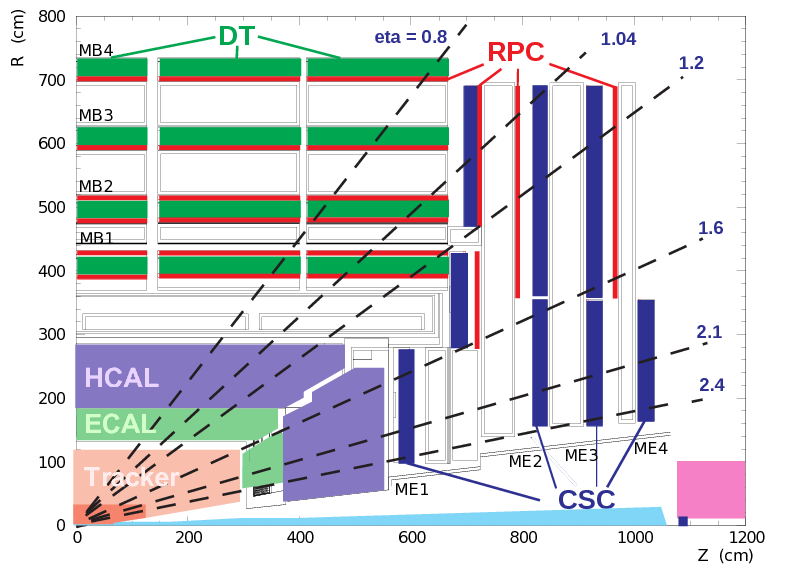
\includegraphics[width=13cm,height=8cm]{ch2/figures/cmsMuonSystem.png}
 \caption{A schematic design of one quadrant of the muon system in the $r-z$ plane showing the position of three sub-detectors used for muon detection~\cite{Web:CERNcds}.}
 \label{fig:cmsMuonSystem}
\end{figure}

\subsubsection{Drift Tube Chambers}
In the barrel region, where the muon flux is low and the magnetic field uniform, four layers of muon stations are used, occupied by drift tube (DT) 
chambers covering up to $\abs{\eta}<1.2$. The three innermost stations are comprised of 12 chambers each, which measure muon coordinates in the $r-\phi$ plane and provide a measurement in the $z-$direction, while the outermost station measures only the 
$\phi-$view. The DT chambers 
consist of individual drift tube cells that contain a 50\unit{\mu{m}} diameter anode wire and two electrode plates that
 create the drift electric field. The walls of the cell are grounded, acting as cathodes. 
%The drift cells of each chamber are 
%offset by a half-cell width with respect to their neighbors so as to eliminate dead spots in the efficiency. 
The cells are filled with a gas mixture (85\% Ar and 15\% CO$_{2}$) and the wire and electrodes are operated with a voltage difference of 
about 1.8\unit{kV}. The transverse dimension of the cells was chosen to be 21\unit{mm} to optimize drift time, gain and number of channels. 
With these design parameters, the DT achieve a gain of 10$^{5}$, resulting in a drift time of 380\unit{ns} and a linear relationship between 
drift time and drift path which is essential for the chamber to provide triggering capabilities. \Fig{\ref{fig:cmsDT}} shows the basic design 
of a DT cell. 

\begin{figure}[h!]
 \centering
 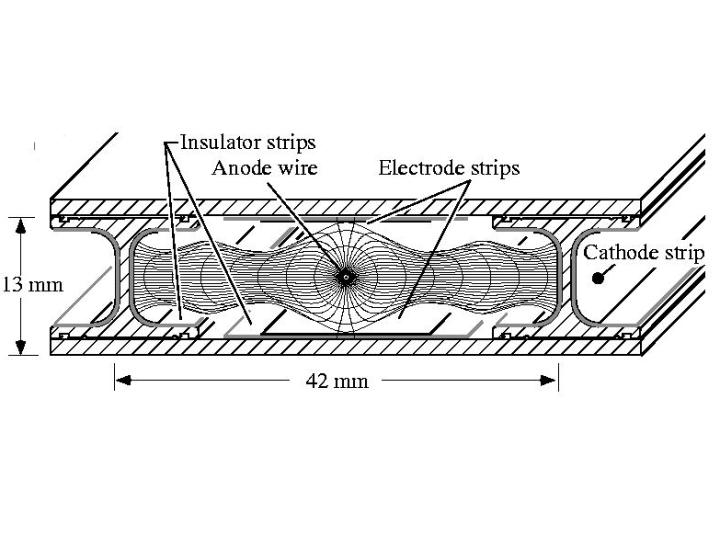
\includegraphics[width=13cm,height=8cm]{ch2/figures/DT.jpg}
 \caption{Individual drift tube cells and pictorial representation of its operation principle~\cite{cmsTDR}.}
 \label{fig:cmsDT}
\end{figure}

\subsubsection{Cathode Strip Chambers}
In the endcap regions, where the magnetic field is large and non-uniform, cathode strip chambers (CSC) are installed providing a coverage in the 
region $0.9<\abs{\eta}<2.4$. The CSCs are multi-wire proportional chambers consisting of six planes of anode wires interleaved among seven cathode 
panels. The gold-plated tungsten wires run azimuthally, defining the track's radial component, while the strips are milled on cathode panels and run 
lengthwise at a constant \dphi width. The angular ($\phi$) position of the track is estimated by extrapolating the charge that is induced on the 
strips as shown in \fig{\ref{fig:cmsCSC}}. The nominal gas mixture is 40\% Ar, 50\% CO$_{2}$ and and 10\% CF$_{4}$. Addition of CF$_{4}$ helps to 
avoid polymerization on wires. The wires give very fast signals that provide very good time resolution while the development of the avalanche on 
the strips gives very good position resolution. The CSCs can operate at high rates and in large and non-uniform magnetic fields without requiring 
precise monitoring of gas, pressure or temperature and can provide trigger and precision position measurement in the same device. The CSC system 
comprises of 468 trapezoidal chambers covering 10$^{^{\circ}}$ or 20$^{^{\circ}}$ in the $\phi-$direction.
\begin{figure}[h!]
 \centering
 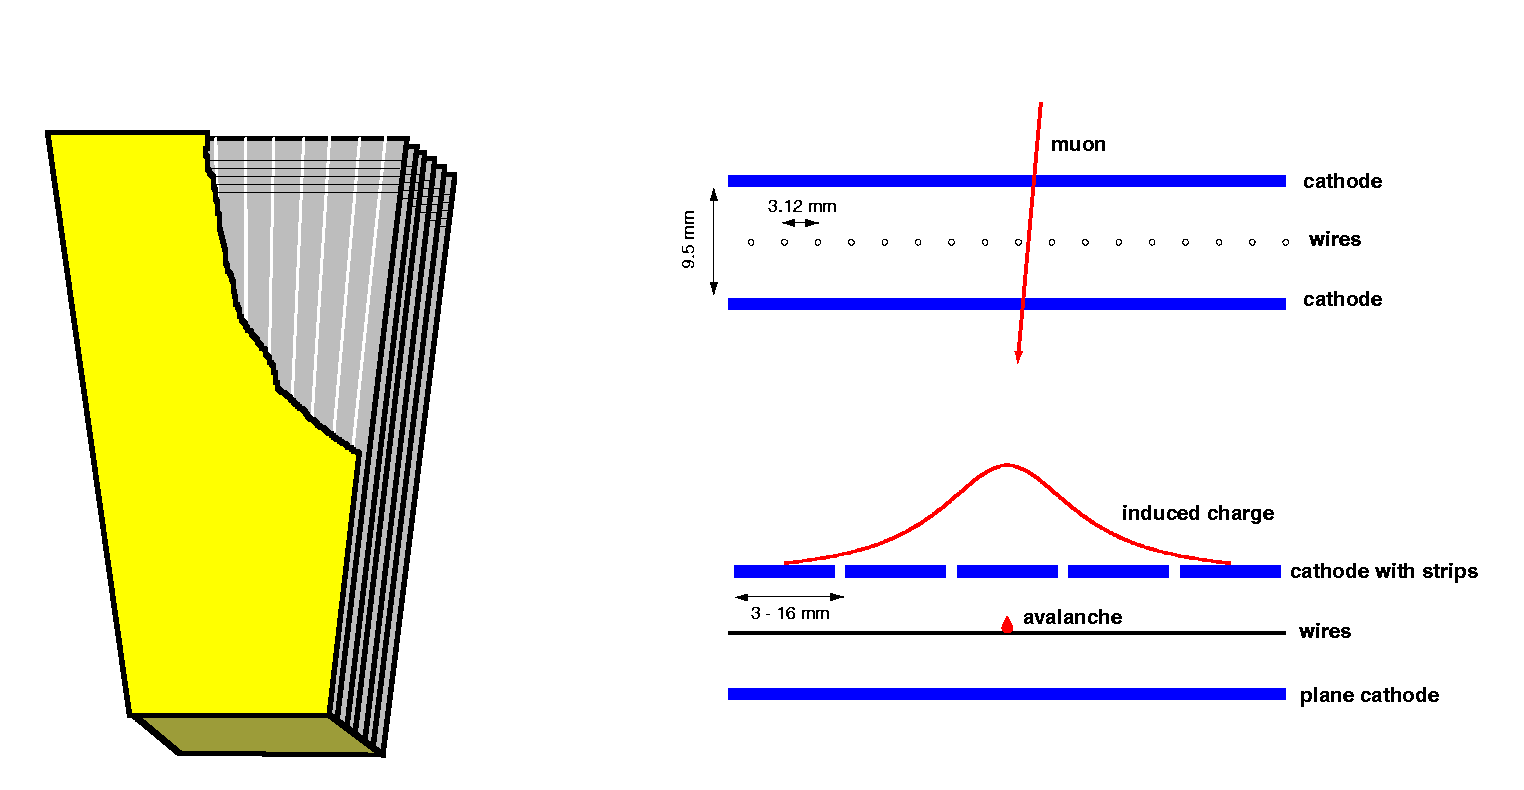
\includegraphics[width=13cm,height=8cm]{ch2/figures/csc.png}
 \caption{Operation principle of the Cathode Strip Chamber~\cite{Web:CERNcds}.}
 \label{fig:cmsCSC}
\end{figure}

\subsubsection{Resistive Plate Chambers}
In order to improve the performance of the muon trigger, an additional system of resistive plate chambers (RPCs) is installed, spanning both the 
barrel and the endcap regions. The RPC system has 480 barrel and 432 endcap chambers. Two rectangular section RPCs per DT chamber are installed 
in the barrel region and two trapezoidal ones per CSC chambers are installed in the endcap regions. They are parallel plate gaseous detectors that 
combine adequate position resolution with a very high operational speed. The RPC is able to tag the presence of an ionizing particle in a time-frame
much shorter than the typical bunch crossing time, which makes it an ideal trigger device since, together, they can associate the correct bunch 
crossing (25\unit{ns} between two bunch crossings) with the muon. The CMS RPC chamber consists of two gaps operated in an avalanche mode with read-out 
strips in-between. The total induced signal is the sum of the induced signal in both gaps. The RPCs need intensive monitoring of temperature, humidity 
and pressure to ensure stability of conditions for proper operation. 

The CMS muon system consists of about 25000\unit{m^{2}} of detection planes and about a million readout channels. For a stand 
alone muon system, for \pt up to 200\unit{GeV} at low $\eta$, the offline muon momentum resolution~\cite{Chatrchyan:2008aa} is $\sim 9\%$ 
(due to multiple scattering in the detector material before the first muon station). It however, varies between $15-40\%$ at 
$\pt\sim1\unit{TeV}$ depending on $\eta$. Adding information from the inner tracker, \ie, considering a global muon, improves the
momentum resolution by an order of magnitude at low \pt. At high \pt (1\unit{TeV}) the global muon has a momentum resolution of about 5\%.

\section{Trigger and Data Acquisition Systems}\label{Se:triDas}
At the nominal design LHC luminosity of $10^{34}\unit{cm^{-2}s^{-1}}$, a bunch crossing rate of 40\unit{MHz} (or 25\unit{ns}) will result in 
$\sim10^{9}$ interactions per second, leading to $\sim100\unit{TB}$ of data to be stored. It is, thus, almost impossible to store information about 
each interaction for offline processing. Hence, for reducing the data in real time and still keeping potentially interesting events, an 
automated system, commonly referred to as the  trigger system~\cite{triggerTDR} is designed along with a Data AcQuisition (\gls{DAQ}) system~\cite{daqhltTDR}
to operate at the unprecedented LHC rate. The frequency of events to be recorded for offline processing is of the order of a few 100\unit{Hz}
achieved by the two-layer trigger system. The first is a Level-1 trigger (L1), implemented in the hardware, based on custom electronics and is
 designed to reduce the incoming average data rate to a maximum of 100\unit{kHz}. The second level, called High Level Trigger (\gls{HLT}), is a software 
based decision taking system, relying on thousands of commercial processors in an event filter farm. The data event passing both levels of
triggering system is recorded for offline physics analysis. A brief description of the L1 and HLT systems is given in sections to follow. 
%The function of the trigger system is not only to reduce the event rate to be written to the tape, but also to segregate events into different type of datasets such as photon, electron, jet datasets, etc. 
\begin{figure}[h]
\centering
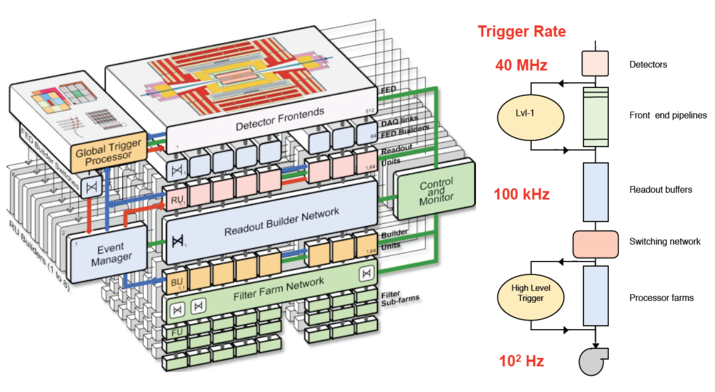
\includegraphics[width=15cm,height=8cm]{ch2/figures/DAQsystem.png}
\caption{Schematic diagram of architecture of CMS DAQ and trigger system~\cite{Web:CERNcds}.}
\label{fig:DAQsystem}
\end{figure}
To reduce the output rate further, at both the L1 and HLT levels, algorithms can be $prescaled$ to accept only a fraction  of the events which pass the 
selection criteria defined by a specific algorithm. The HLT is a part of the DAQ system that manages the overall flow of the data. The DAQ system also 
includes detector front-end electronics, readout modules, an event builder network, as well as management and monitoring systems. The diagram of the 
complete DAQ system along with the trigger system is shown schematically in \fig{\ref{fig:DAQsystem}}.

\subsection{Level-1 Trigger}
The L1 trigger~\cite{triggerTDR} is implemented in the form of custom hardware processors which use only low resolution, coarsely segmented
data from calorimeters and muon systems while holding the high resolution data in pipelined memories in the front end electronics. The L1
pipeline data storage time is 3.2\unit{\mu{s}}, the time in which the L1 trigger decision is transmitted to the detector electronics. The
purpose of the L1 trigger is to perform sufficient reduction from the input crossing rate of $\sim40\unit{MHz}$ to provide an output rate of few 
100\unit{kHz}. The hardware components of the L1 trigger consist of field-programmable gate-array (FPGA) technology, as well as ASICs and programmable lookup tables (LUTs).

A block diagram depicting the schematic overview of the L1 trigger system is shown in \fig{\ref{fig:L1trigger}}.
At each bunch crossing, the calorimeters produce separate ECAL and HCAL trigger primitives based on energy deposited in the respective calorimeters,
which are then processed in the Regional Calorimeter Trigger (\gls{RCT}) before being sent to the Global Calorimeter Trigger (\gls{GCT}). The GCT sorts electron, 
photon, and jet candidates (including jets coming from hadronic decays of $\tau$ leptons) and calculates global quantities like \met and \HT which
are fed into the CMS Global Trigger (\gls{GT}).
\begin{figure}[h]
\centering
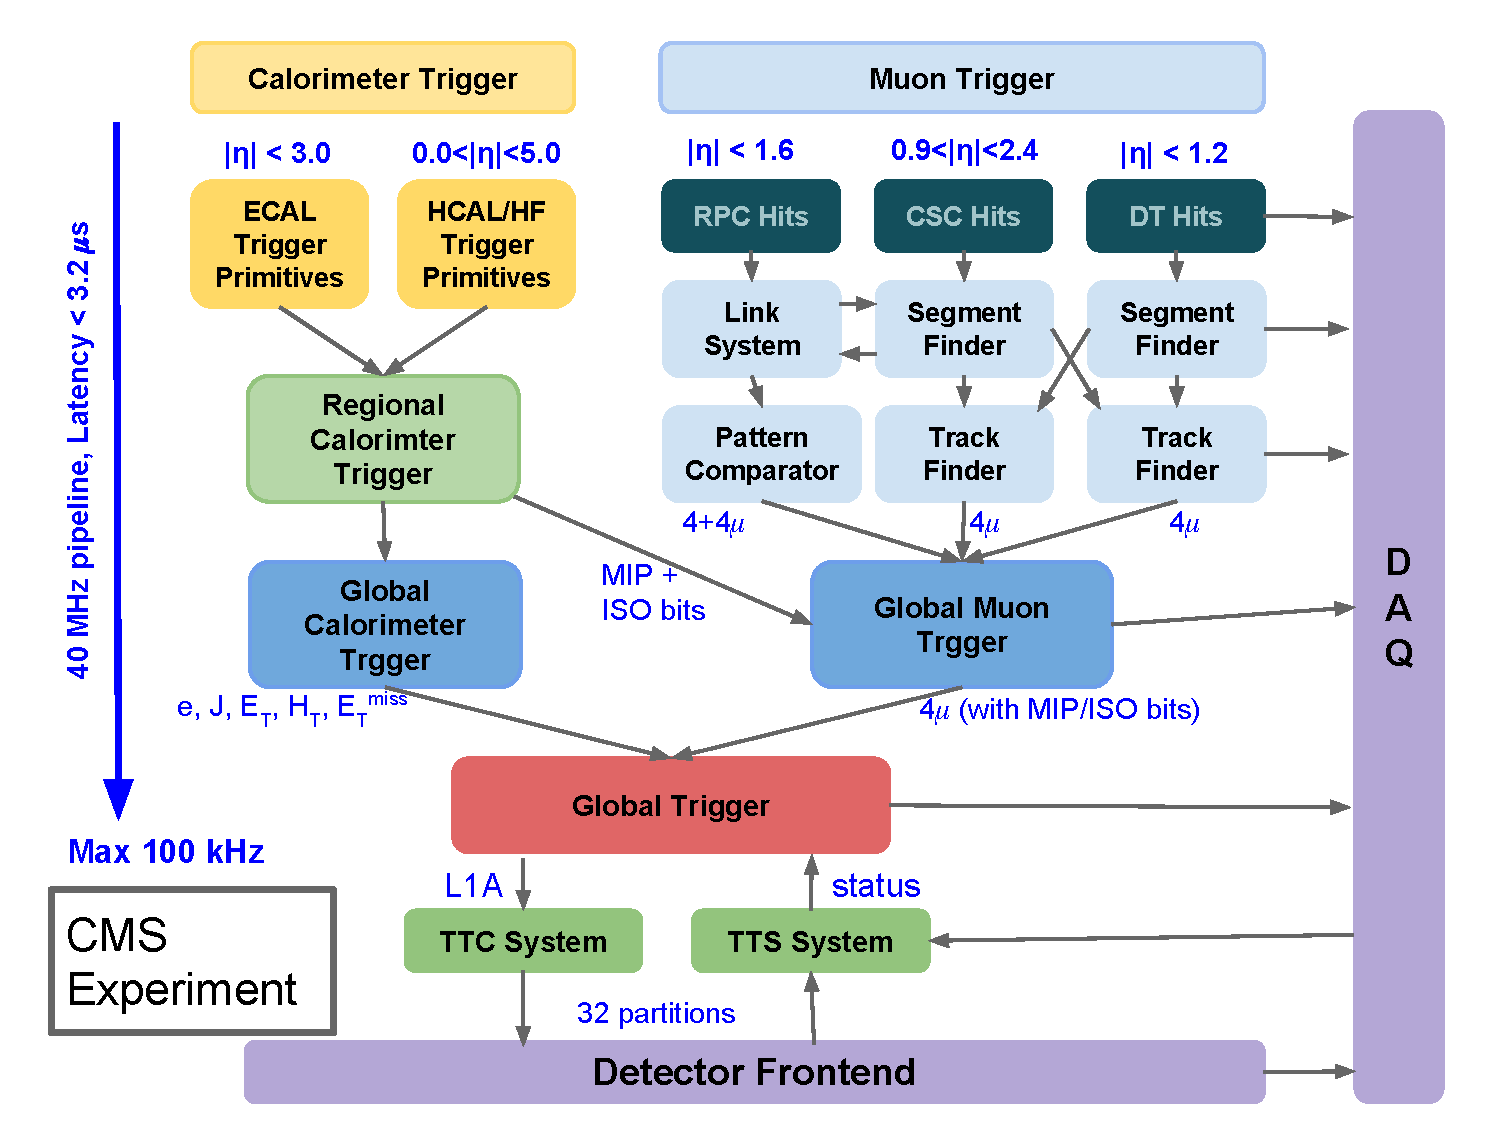
\includegraphics[width=14cm,height=8cm]{ch2/figures/L1Trigger_BlockDiag.pdf}
\caption{Architecture of CMS Level-1 trigger system~\cite{triggerTDR}.}
\label{fig:L1trigger}
\end{figure}
In muon subsystems, the DTs and CSCs create the track segments using the hit patterns in the chambers and send them to a track-finder to select 
the top 4-muon  candidates per subsystem. The RPCs, using a different approach, compare patterns of 4-barrel and -endcap muons. Exchanging track 
segments information among muon subsystems helps close geometric gaps in the muon coverage and raise overall muon trigger efficiency. Finally, 16 
muon candidates are passed to the Global Muon Trigger (\gls{GMT}) system for sorting and removal of duplicates. The GMT then sends the top 4-global 
muon candidates taking information from the RCT on calorimeter deposits around the muon candidates enabling the use of isolated muon triggers to GT. 

The GT receives all the trigger objects from GCT and RCT systems. It then applies programmable topological cuts and different energy thresholds on 
these objects and issues the final Level-1 Accept (L1A) decision. The L1A is then sent to the Trigger Timing and Control (\gls{TTC}) system for distribution 
to the detector front-end electronics. The TTC interfaces with the LHC to provide orbit and clock information. The GT sends out command via the TTC to 
keep the detectors and their electronics and all the links in sync, stop a run, start a run, etc. 

\subsection{High Level Trigger}
The High Level Trigger (HLT)~\cite{daqhltTDR} receives and processes the events accepted by the L1 trigger by using a software based system
composed of an event filter farm of commercial CPUs with filters and builder units. The goal of the HLT is to reduce the incoming rate of 
100\unit{kHz} by a factor of $\mathcal{O}(10^{3})$, leading to an output rate of the order of few 100\unit{Hz}. 
The HLT makes use of full resolution and granularity of the detector to run complex algorithms for offline reconstruction of the events.
The average processing time is roughly 40\unit{ms}, with some events requiring up to a second. 
At this stage, the information from the tracker is also used for isolation and trigger selection. The full event information is analyzed via a 
predetermined set of algorithms with programmable structures and thresholds known as \emph{trigger paths}, constituting a \emph{trigger menu}.
A \emph{trigger path} is nothing but a set of algorithms that reconstruct one or more physics candidates and applies selection criteria to these
 reconstructed candidates and their various isolation and kinematical quantities. The algorithms in each path are executed in increasing order
of complexity to reduce the input rate before CPU-expensive reconstructions, such as the particle-flow algorithm. Events satisfying any one of the HLT 
trigger paths are sent to the storage manager where the event data is stored locally on disks until transferred to the CMS Tier-0 center at CERN
for offline processing and permanent storage. More details about the HLT designed for this analysis are prescribed in \chap{\ref{ch:QstarAnalysis}}.

\subsection{DAQ}
The CMS Data Acquisition System (DAQ)~\cite{daqhltTDR} collects data fragments from respective detector front-ends to form a full
event in two stages before transporting them between the L1, HLT, and the storage center. The architecture of the CMS DAQ is schematically
shown in \fig{\ref{fig:DAQsystem}}. It sustains an input rate of 100\unit{kHz}, for a data flow of about 100\unit{GB/s}. It provides
necessary computing power for the HLT to perform its operations. The DAQ system utilizes up to eight slices that work autonomously
and can handle an event rate up to 12.5\unit{kHz}. The Trigger-Throttling-System (\gls{TTS}) is designed to protect the system against the back-pressures, 
which may occur when the buffer overflows in the sub-detectors Front-End Drivers (\gls{FED}) due to variation in event size or rate, leading to loss of 
synchronization. The TTS gives a quick feedback from any sub-detector FEDs to the GT processor to control trigger rates before the buffer overflows. 
Furthermore, \emph{prescales} could be adjusted to optimize the available DAQ capacity and performance during operation.

\section{Software and Computing}\label{Se:Software}
The CMS users have access to a collection of softwares of the CMS experiment based on object oriented structures in C++ and python, referred to,
in the whole, as the CMS software framework (CMSSW)~\cite{cmsTDR}. The single framework supports a variety of applications covering the entire range of 
experimental work including simulation, calibration and alignment, and reconstruction modules that process event data in order to perform
physics analysis. The CMSSW event processing model is composed of one executable, know as cmsRun, and various plug-in modules that are
managed by the framework. All the codes needed in the processing of events (calibration, reconstruction algorithms, etc.) are contained
in the modules. The same executable is used for both the detector and Monte Carlo (MC) simulated data. 

The CMS offline computing system has to support the storage, transfer and manipulation of the recorded collision data. The CMS application software
performs a variety of event processing, selection and analysis tasks. The main concept of the CMS data model is the ``Event''. The ``Event'' provides
access to the information stored in the recorded data. The ``Events'' are physically stored as ROOT files. The ``Event'' is used by a variety of
 physics modules which perform well-defined functions of reconstruction or analysis of the Event. The modules execute independently from one another.

The CMS computing system has several event formats with differing levels of detail and precision in order to achieve the required level of 
data reduction. The RAW format contains the full recorded information from the detector and also a record of the trigger selection. The RAW
data is permanently archived in safe storage with size of 1.5\unit{MB/event}. For simulated data, the size of the RAW dataset is about 2\unit{MB/event}
due to additional Monte Carlo information. The Reconstructed (\gls{RECO}) data is derived from the RAW data and provides access to reconstructed physics
objects for physics analysis in a convenient format. The RECO events contain high-level physics objects such as jets, photons, muons, electrons, 
\bjets, etc, with a size of the order of 250\unit{kB/event}. The Analysis Object Data (AOD) is the compact analysis format with a reduced size of 
$\sim50\unit{kB/event}$, which is produced by filtering of RECO data to be used by almost all the physics analyses.
%\bibliography{ch2/ch2_ref} %% defined in main file
